\section{Signal efficiency}
\label{sec:signal}

We search for several models of heavy resonances decaying to
a W or Z boson on one side, and a Higgs on the other, where both bosons 
decay to quarks producing merged jet.  This analysis is focused on two
channels:
\begin{itemize}
\item \HbbVqq, and
\item \HwwVqq
\end{itemize}
As previously discussed, we use one V-tagging and two Higgs tagging algorithms
to identify such events.  After subdividing the events according to 
high purity and low purity tags, we end up with five distinct categories,
as shown in Table~\ref{table:categories}.

In this section, we discuss various issues related to the evaluation
of the signal efficiency.

% For Higgs decays to \bbbar, we use a pruned jet mass and also b
% tagging to discriminate higgs jet from QCD jets and jets from the
% fully merged hadronically decaying top quark.
% Fig.~\ref{fig:JetMassTagging} shows the pruned jet mass distribution for
% Higgs jet, $\Zqq$ jet, hadronic top jets and QCD jets.


%HbbZqqfigs/Signal



%% &&& Plot:  the pruned jet mass of Higgs Jet and QCD jet , Z jet, top jet? in one plot. 

%% &&& Plot:  tau42 for Higgs Jet , Z jets, WJets, top jet, in one plot. leptonic top jet ?


%The pruned jet mass and jet $\tau_{21}$ distributions in signal MC, data and background MC are shown in Fig.~\ref{fig:taggingvariables}.



\subsection{Cross-talk between the Higgs decay channels}
\label{sec:cross-talk}

In order to combine events from all categories into a single joint
likelihood, the categories must be mutually exclusive.  However, a
cross-talk between the Higgs channels is neverthelss possible: for
example, $\Hbb$ tagger can identify other two-prong Higgs decay modes
like ${\rm H\to gg}$, $H \to \tau \tau$, or ${\rm H \to c\bar{c}}$,
although this kind of `false positive' tag happens only rarely (the
efficiency is $\lesssim 6~\%$).  Similarly, events from two-prong
Higgs decay channels can also pass the $\tau_{42}$ cut in the
$\Hww$ selection.  In this case, the channel $\Hbb$, because of its large
branching ratio, contributes a non-negligible number of events to the
sample of 4q tags.  This effect is illustrated by
Fig.~\ref{fig:HiggsTau42}, where it can be seen that most of the
low-$\tau_{42}$ tail of the $\Hbb$ curve will be below the cut value of 0.55.
\begin{figure}[htb]
\centering
\begin{tabular}{cc}
%     \resizebox{0.5\linewidth}{!}{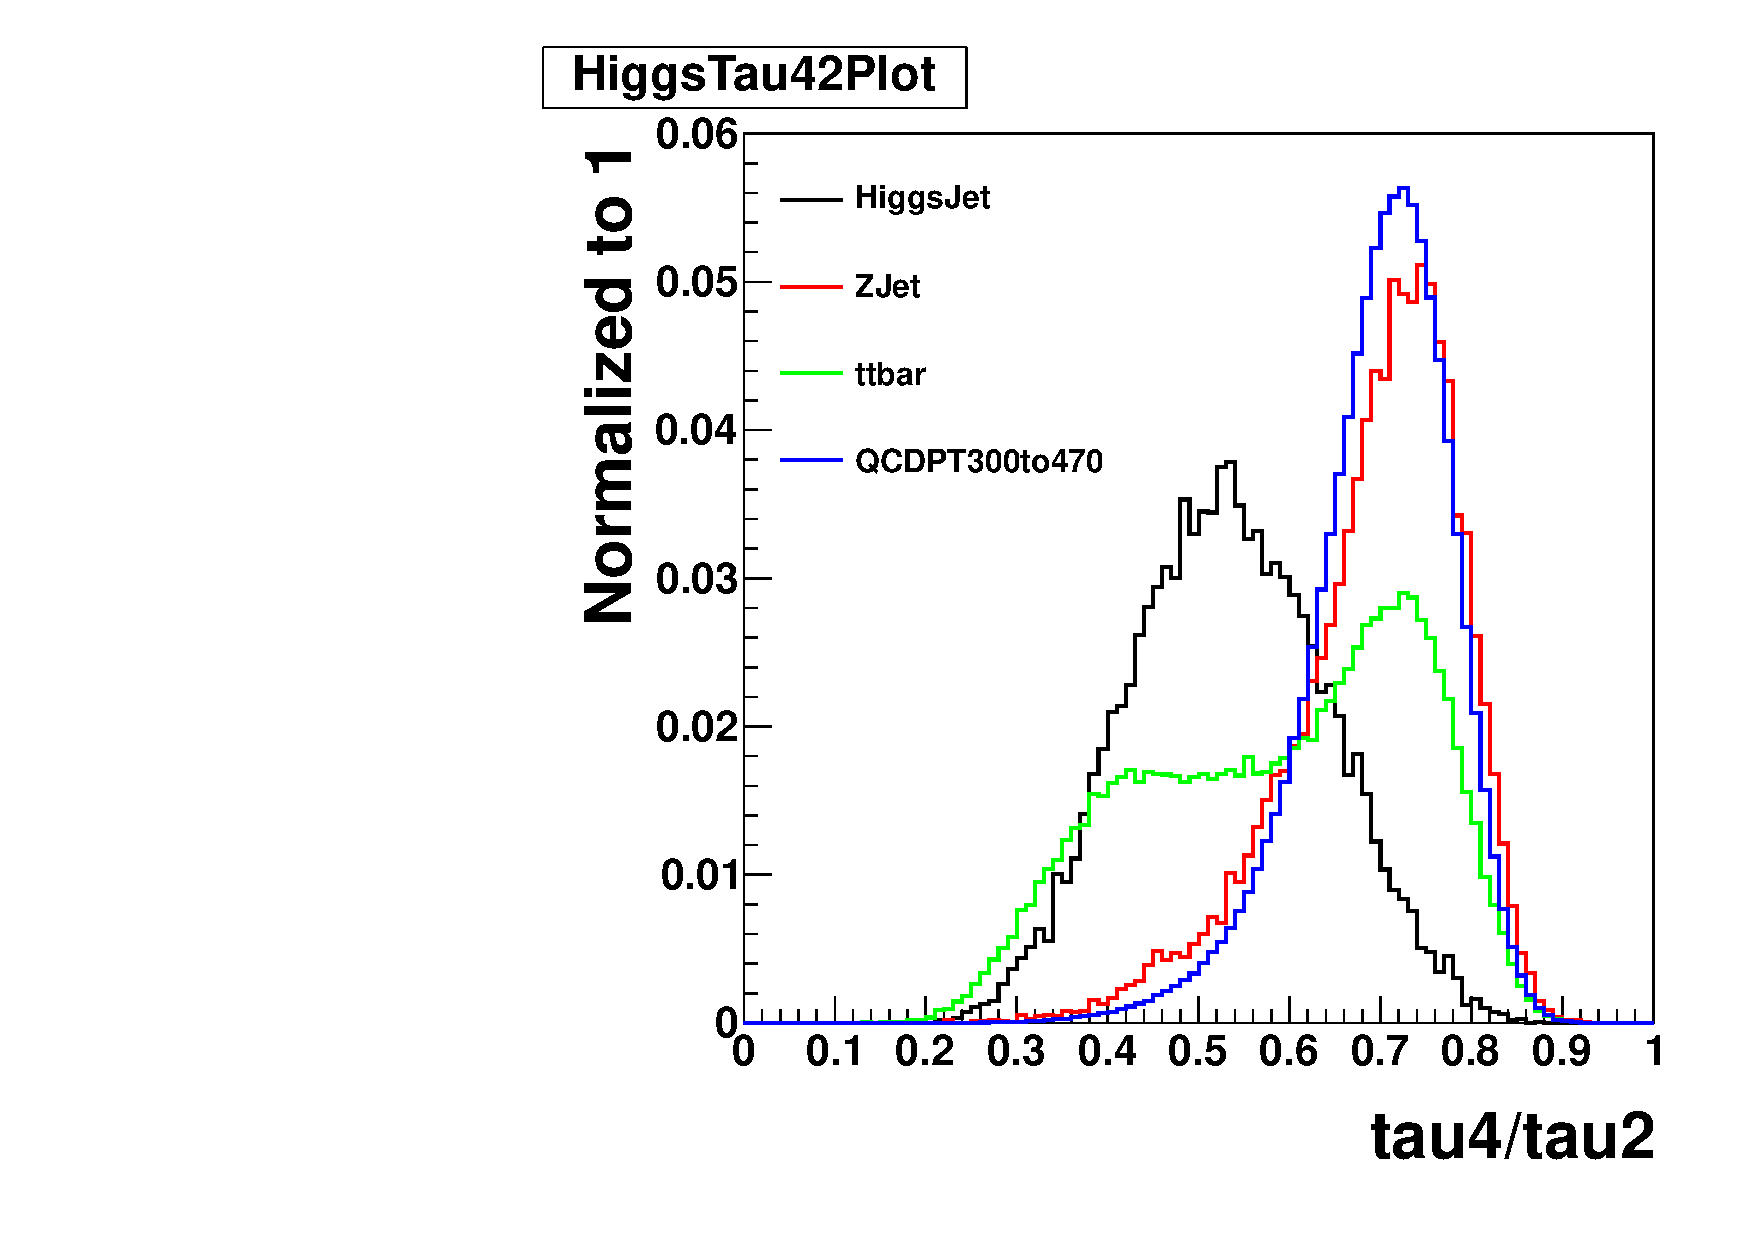
\includegraphics{HqqqqZqqfigs/N-subjettiness/Tau421TeVPre.pdf}} &
     \resizebox{0.7\linewidth}{!}{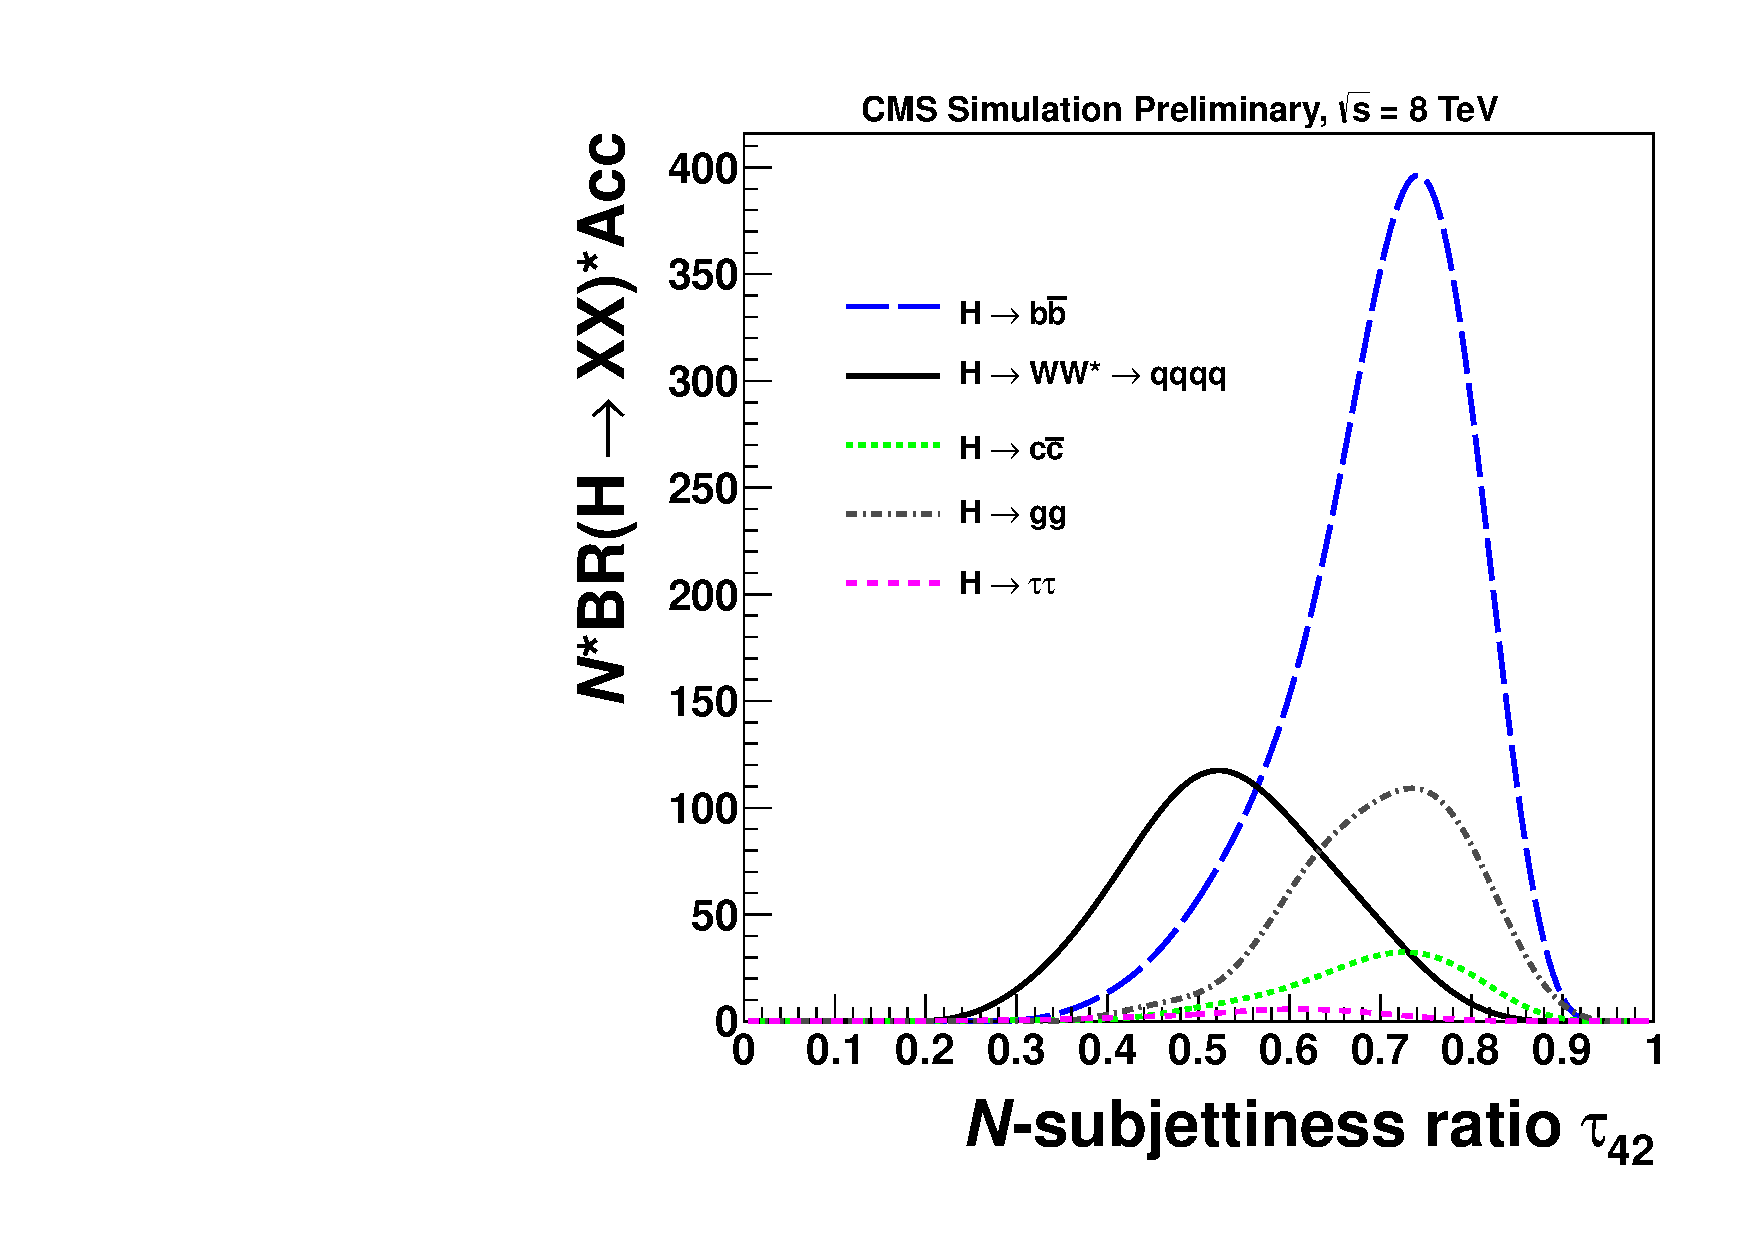
\includegraphics{EXO-14-009/HqqqqZqqfigs/cross-talk/cross-talk.pdf}} \\
\end{tabular}
\caption{ Comparison of $\tau_{42}$ distribution for H(ww$\to qqqq$), H(gg), H(bb), H(cc), H($\tau\tau$) channels.
All curves are drawn for Higgs jets after pruned jet mass cut, and also normalized with 
respective branching ratios.}
\label{fig:HiggsTau42}
\end{figure}
 

%\newpage
%\section{Hbb HWW and other Channels}
%\label{sec:contamination}

Table~\ref{table:HbbHww} provides an overview of the cross-talk
between the various channels.  The Higgs branching ratios correspond
to the Higgs mass of 125~\GeVcc. 
 For ${\rm H \to WW^* \to 4q }$,
the branching ratio of the hadronic decay of (real) W boson is already 
included, so that the final state is four quarks.
%
The table is normalized to 100,000 standard model Higgs
bosons, and the numbers in the
table show the number of Higgs decays that pass the tagger for each
channel, with the branching ratio taken into account.  For example, 
let us consider ${\rm H \to c\bar{c}}$ channel.  At the Z' resonance
mass of 1~\TeVcc, out of 100,000 Higgs decays,  104 events 
are tagged by the $\Hbb$ tagger  
and  82  pass $\Hww$ tagger but fail $\Hbb$ tagger.
For ${\rm H \to ZZ}$ decays, we take its tagging efficiency the same 
as $\Hww$ signals. So the number of ${\rm H \to ZZ}$ to pass $\Hbb$ and 
$\Hww$ tagger is estimated by 
efficiency of $\Hww$ signal times 
 BR(Hzz)*BR(Zqq)*BR(Zqq) divided by BR(Hww)*BR(Wqq)*BR(Wqq). 

From Table~\ref{table:HbbHww}, it can be seen that for various signal 
resonance masses, the contribution of other decay channels to the 
sample of $\Hbb$ tags never exceeds 6\%. We will assign additional systematics
for the cross-talk.  
%This is smaller than several
%of the systematic uncertainties, and we do not correct for it.

%And also the ratio of other signals, i.e. Htt, Hgg, Hcc to pass $\Hww$
%tagger, is around 14\% of $\Hww$ plus $\Hbb$ decay modes.
%Their contamination in data should be very tiny.  

Since the $\Hbb$ tagger has significantly lower background than $\Hww$,
it takes precedence in selecting events: we first identify the
events that pass the $\Hbb$ tagger, and only if they fail,  we
test them for the presence of the $\Hww$ tag.  

%As a consequence
%of such cascading selection, we divide the signal events
%into three categories:
%\begin{enumerate}
%\item $\Hbb$ decays reconstructed by the $\Hbb$ tagger
%\item $\Hbb$ decays that failed the $\Hbb$ tagger, but pass $\Hww$ tagger
%\item $\Hww$ events that pass $\Hww$ tagger.
%\end{enumerate}
%Each of these categories must be treated as a separate signal
%component in the multi-channel joint likelihood.
%, with the Higgs
%branching ratios as the nuisance parameters.

The effect of the $\Hbb$ tagger veto on the $\Hww$ tagged dijet 
mass distribution
background (data) is shown in Appendix~\ref{appendix:crosstalkData}.
%The fraction of $\Hww$ tags which are also $\Hbb$ tags are small,
%about 3\%, and it is roughly a slowly
% rising slope as a function of the dijet
%invariant mass.


\begin{table}[htbp]
\begin{center}
\caption{Number of Higgs jets falls into two exclusive categories, assuming we have 100,000 SM Higgs (125 GeV) decays to all channels.
$\Hzz$ signals are estimated by its branching ratio times the efficiency of $\Hww$ signals divied by the branching ratio of $\Hww$ channel. }
\begin{tabular}{|l|r|r|r|r|}
\hline
%& \multicolumn{1}{l|}{Branching ratio (\%)} & \multicolumn{1}{l|}{Pass $\Hbb$} & \multicolumn{1}{l|}{Pass $\Hww$} & \multicolumn{2}{l|}{Fail $\Hbb$, pass $\Hww$} \\ \hline
& Branching  & Pass       & Fail $\Hbb$, pass \\
& ratio (\%) & $\Hbb$  &   $\Hww$ \\ 
\hline
1.0 TeV & & & \\
$\Hbb$ & 57.70 & 11871 &  804 \\ %\hline
$\Hww$ & 9.94 & 86 &  2360 \\ %\hline
$\Hzz$ & 1.30 & 11  & 309  \\ %\hline
${\rm H\to c\bar{c}}$ & 3.00 & 104 & 82 \\ %\hline
${\rm H\to} \tau \tau$ & 6.30 & 17 & 37 \\ %\hline
${\rm H\to gg}$ & 10.00 & 14 & 314 \\ 
\hline
\\
1.5 TeV  & & & \\
$\Hbb$ & 57.70 & 11444 &  755 \\ %\hline
$\Hww$ & 9.94 & 228 & 1916 \\ % \hline
$\Hzz$ & 1.30 & 29 & 250 \\ % \hline
${\rm H\to c\bar{c}}$ & 3.00 & 121 & 88 \\ %\hline
${\rm H\to} \tau \tau$ & 6.30 & 12  & 57 \\ %\hline
${\rm H\to gg}$ & 10.00 & 69 & 174 \\ %\hline
% & \multicolumn{1}{l|}{} & \multicolumn{1}{l|}{} & \multicolumn{1}{l|}{} & \multicolumn{1}{l|}{} \\
\hline
\\
2.0 TeV &  & & \\ %\multicolumn{1}{l|}{Braching Ratio (\%)} & \multicolumn{1}{l|}{Pass $Hbb$ tagger} & \multicolumn{1}{l|}{Pass Hww tagger} & \multicolumn{1}{l|}{Fail $Hbb$, pass Hww} \\ \hline
$\Hbb$ & 57.70 & 13816 & 551 \\ %\hline
$\Hww$ & 9.94 & 449 & 1435 \\ %\hline
$\Hzz$ & 1.30 & 58 & 187 \\ %\hline
${\rm H\to c\bar{c}}$ & 3.00 & 228 & 99 \\ %\hline
${\rm H\to} \tau \tau$ & 6.30 & 42 & 74 \\ %\hline
${\rm H\to gg}$ & 10.00 & 157  & 262 \\ \hline
\end{tabular}
\label{table:HbbHww}
\end{center}
\end{table}






%\begin{figure}[htb]
%\begin{figure}[ht]
%\begin{center}
%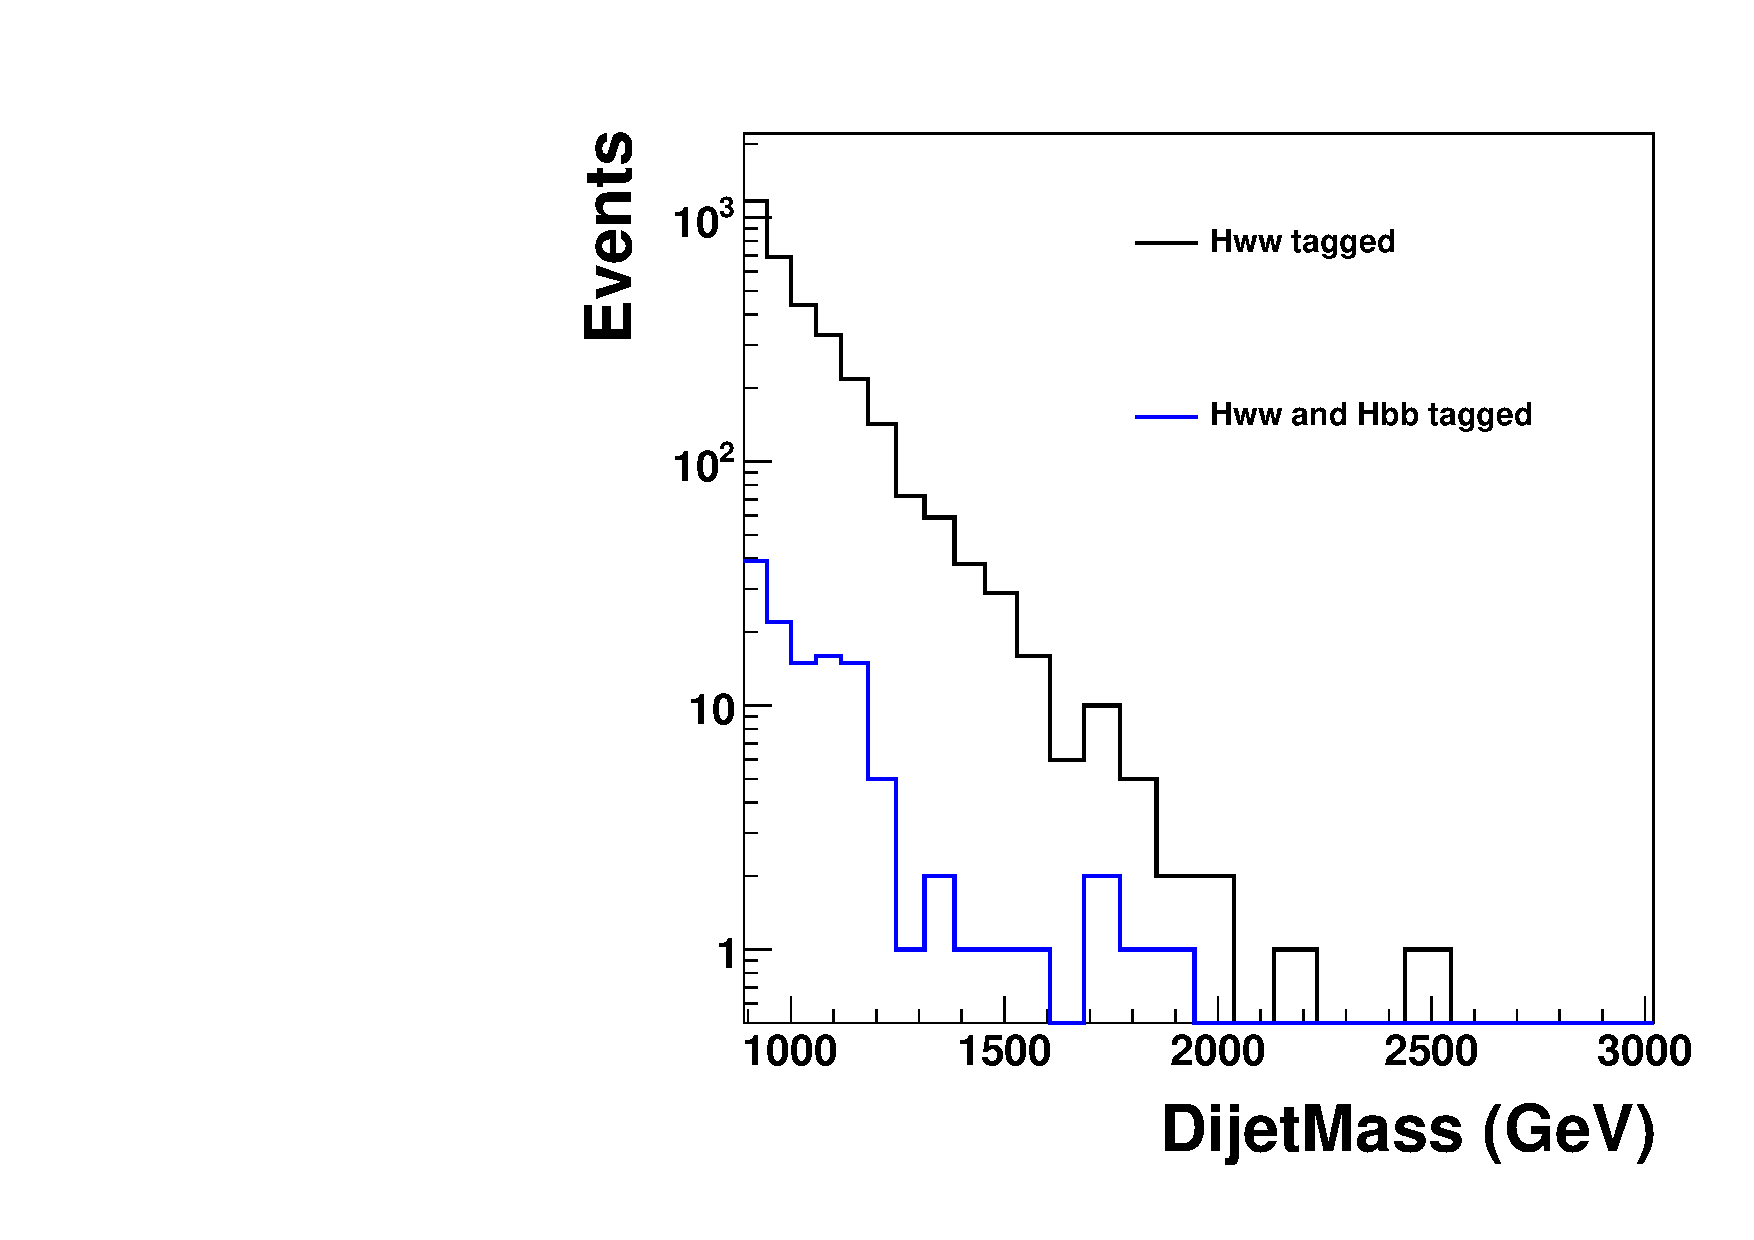
\includegraphics[width=0.49\textwidth, height=0.45\textwidth]{HqqqqZqqfigs/HbbHww/HighPurity.pdf}
%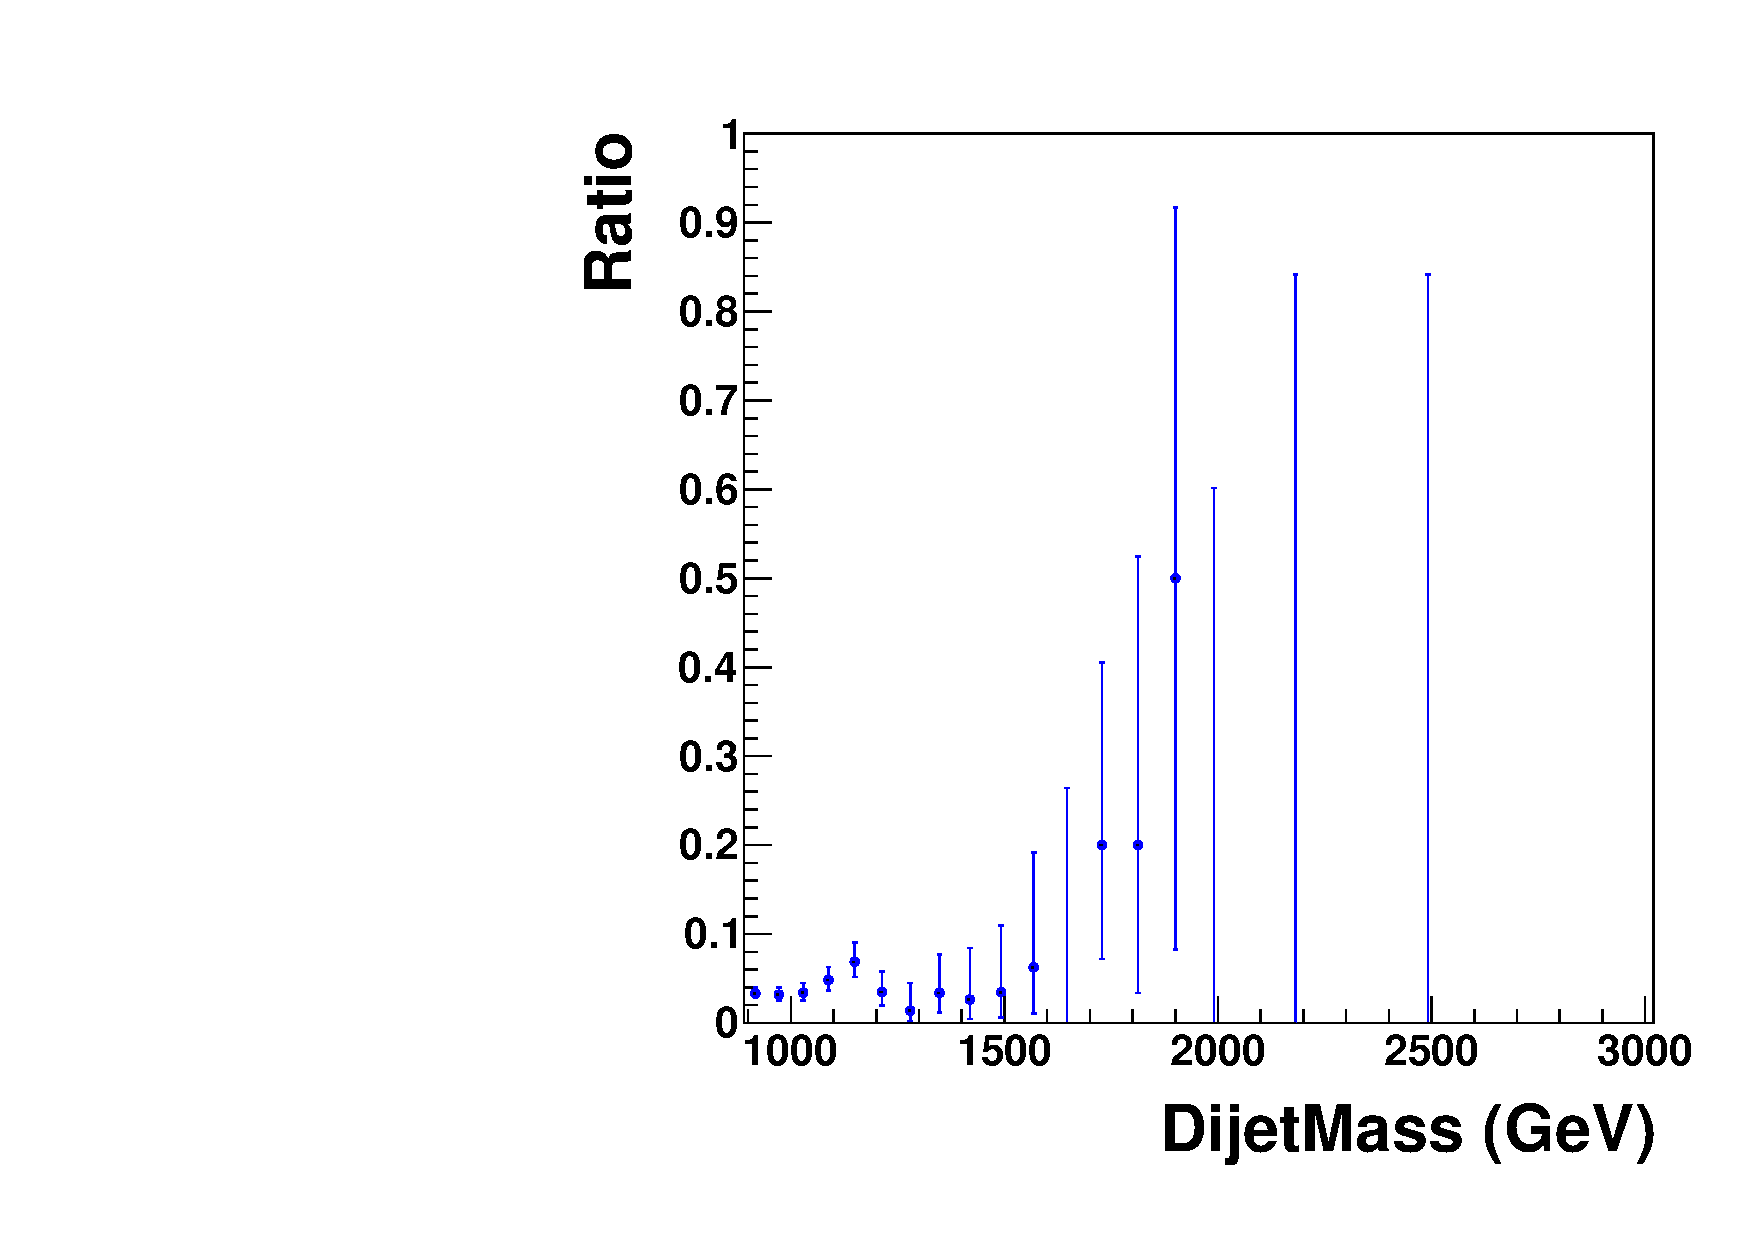
\includegraphics[width=0.49\textwidth, height=0.45\textwidth]{HqqqqZqqfigs/HbbHww/HighPurityRatio.pdf}
%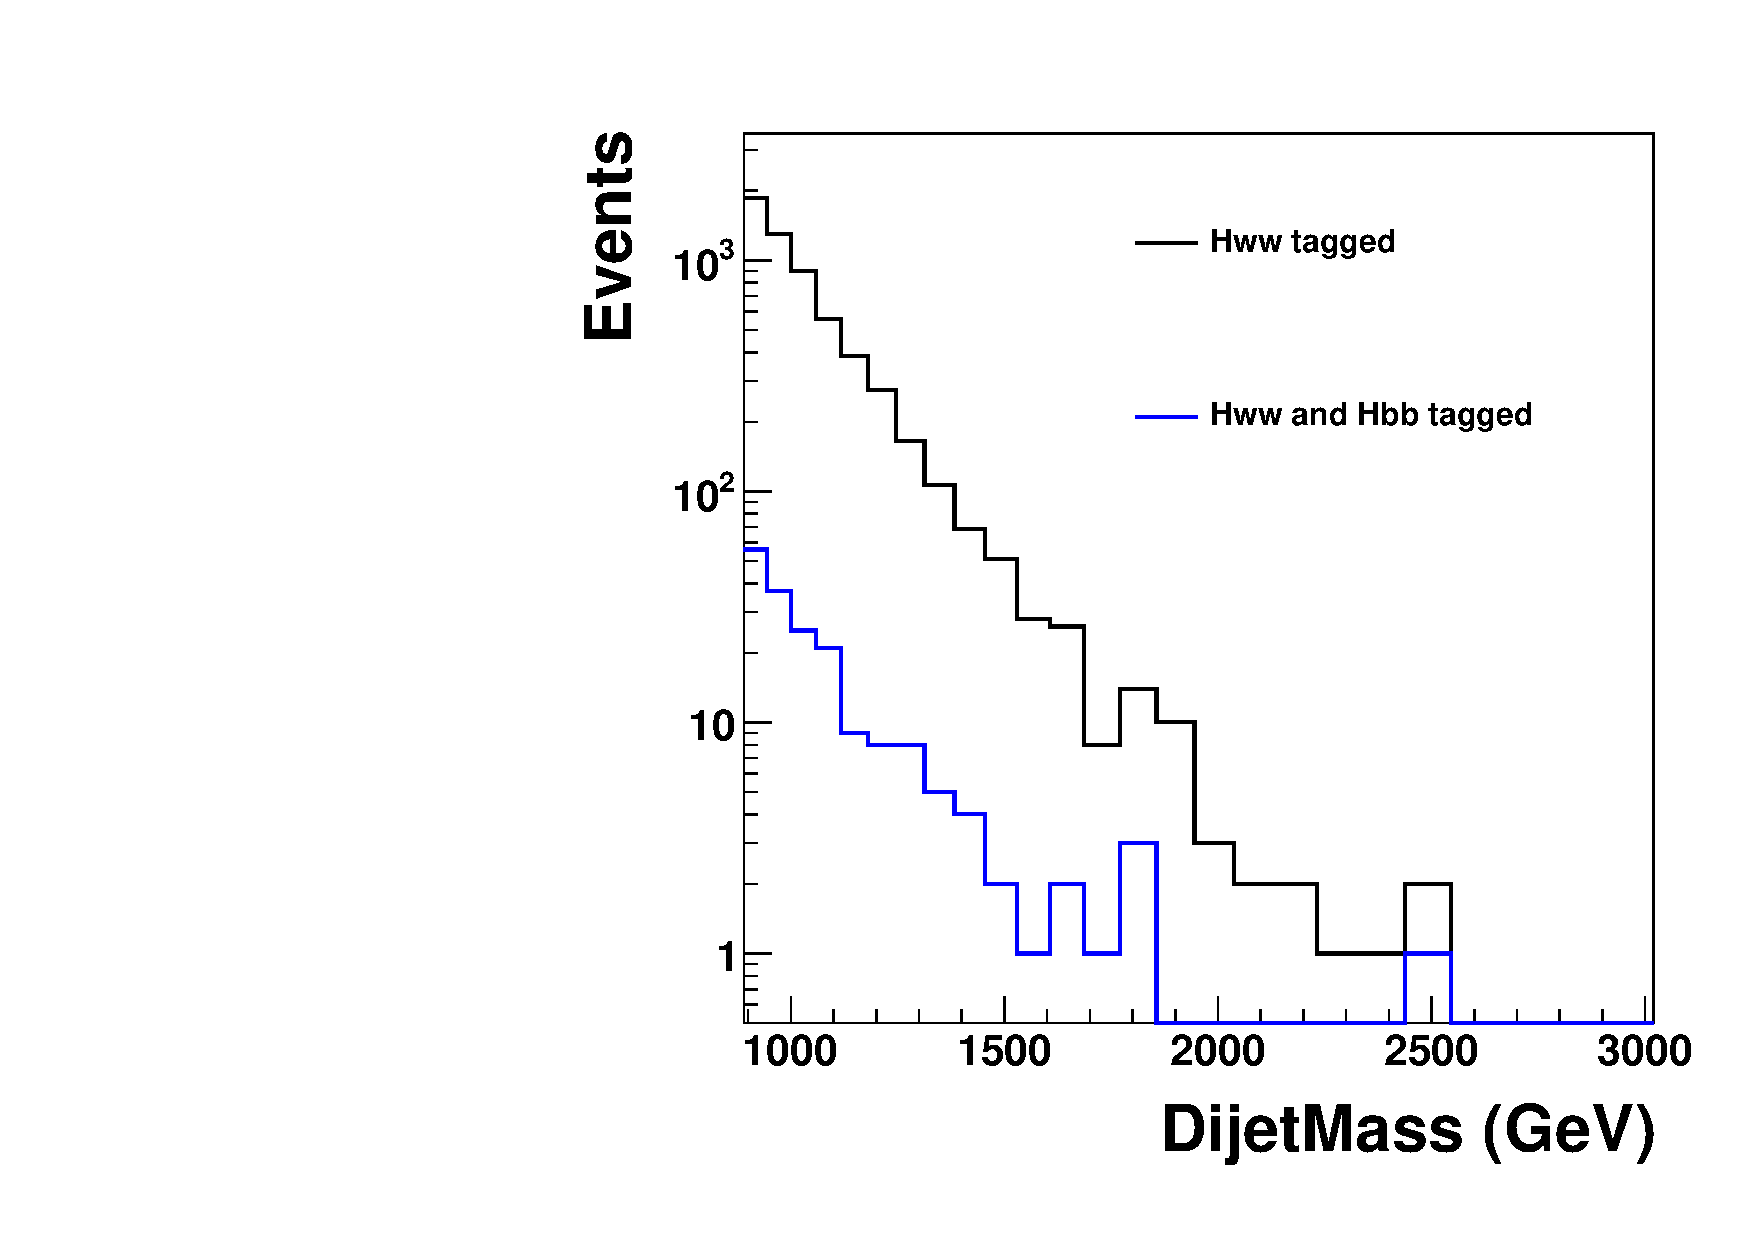
\includegraphics[width=0.49\textwidth, height=0.45\textwidth]{HqqqqZqqfigs/HbbHww/LowHPurity.pdf}
%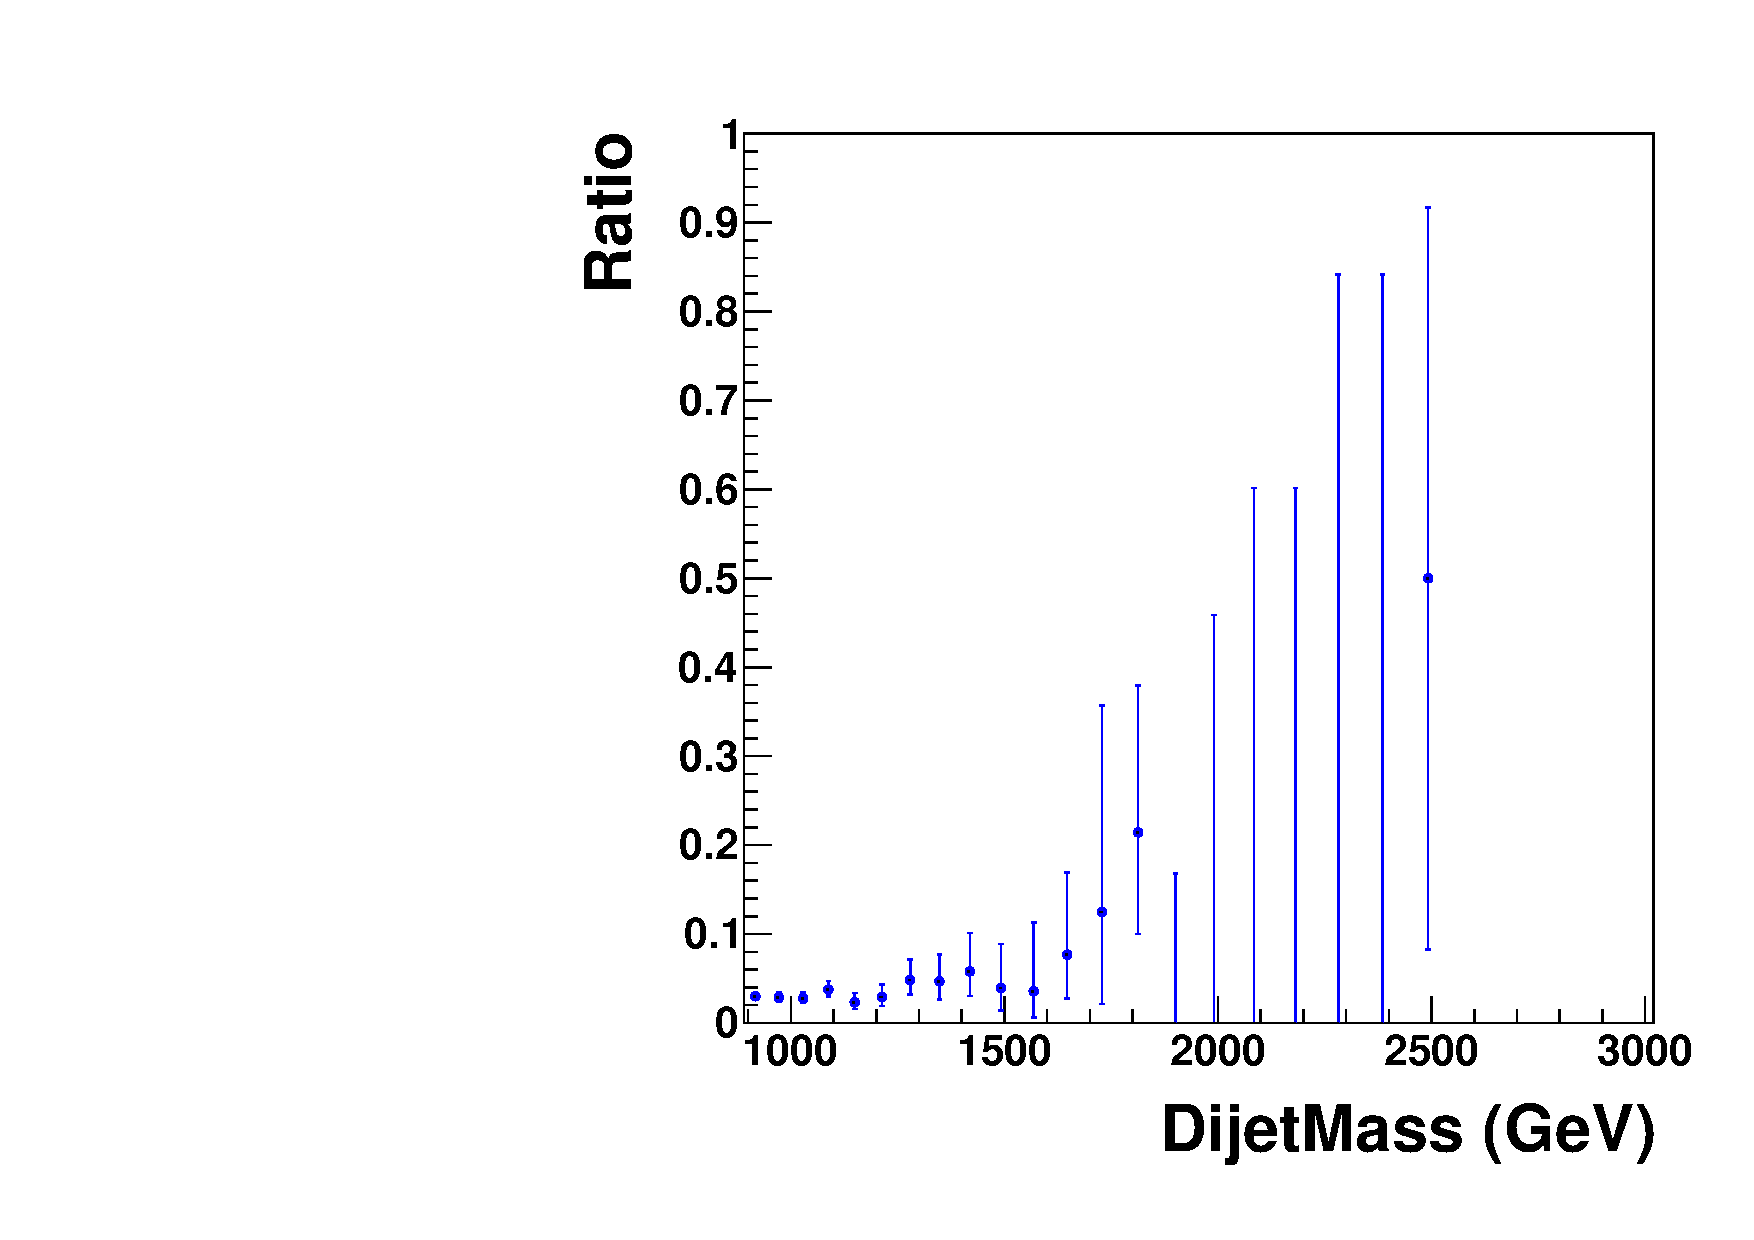
\includegraphics[width=0.49\textwidth, height=0.45\textwidth]{HqqqqZqqfigs/HbbHww/LowHPurityRatio.pdf}
%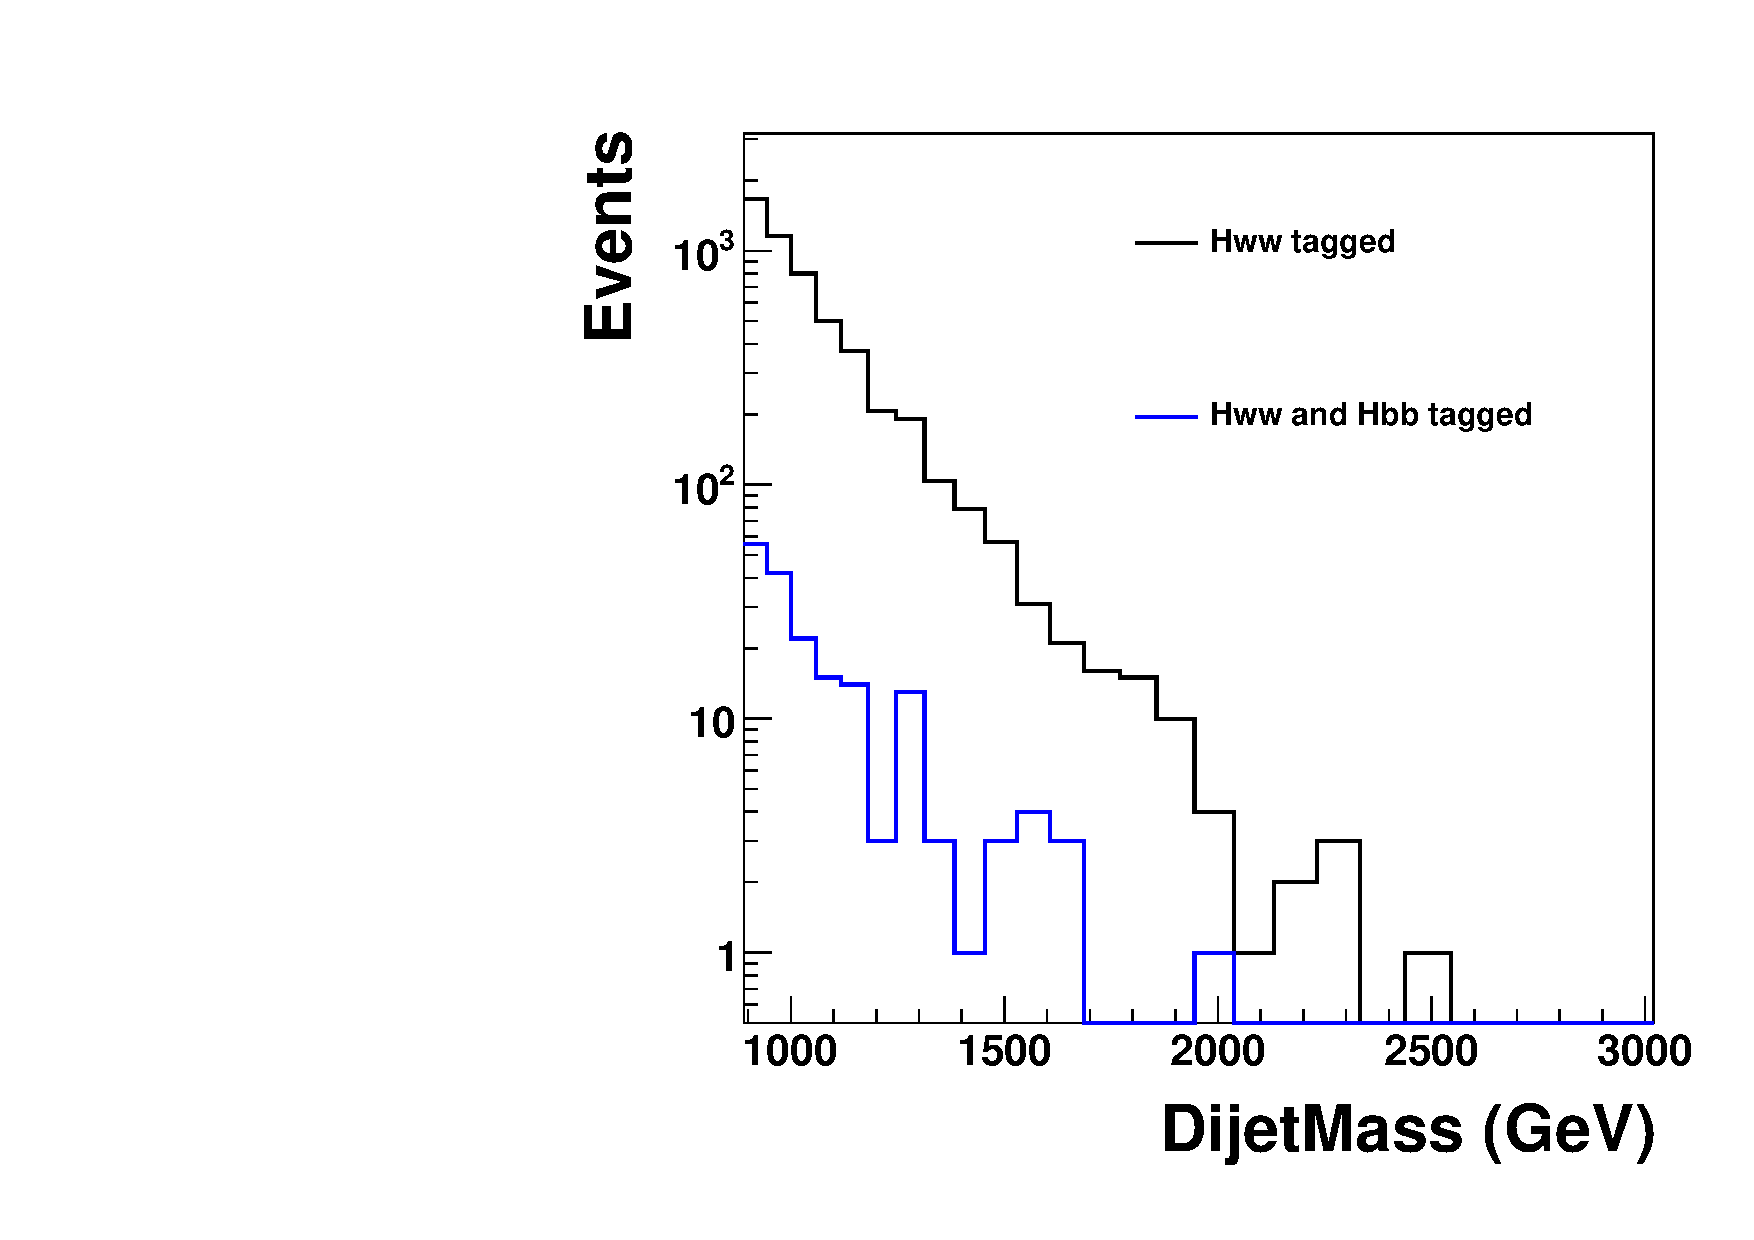
\includegraphics[width=0.49\textwidth, height=0.45\textwidth]{HqqqqZqqfigs/HbbHww/LowVPurity.pdf}
%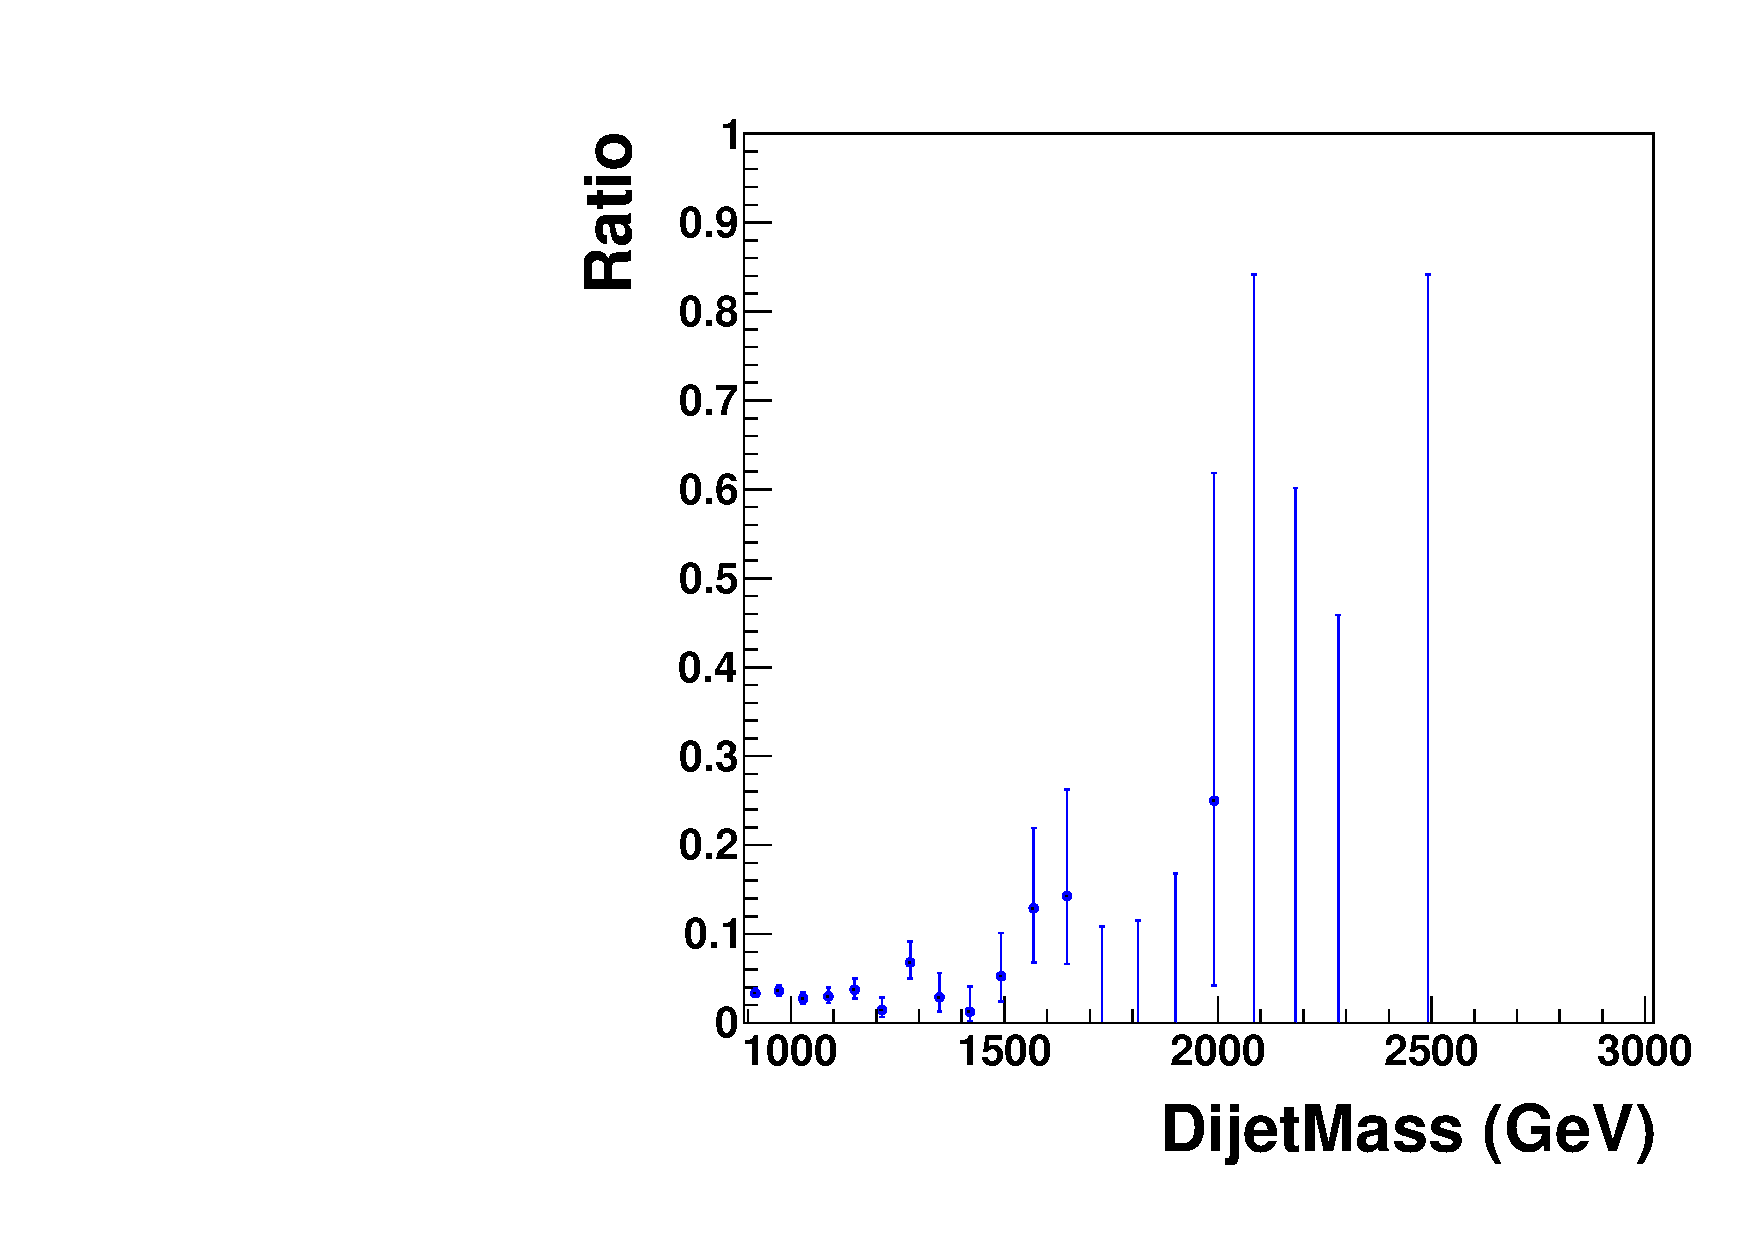
\includegraphics[width=0.49\textwidth, height=0.45\textwidth]{HqqqqZqqfigs/HbbHww/LowVPurityRatio.pdf}
%\end{center}
%\caption{ 
%  Left column: dijet mass distribution in data, for events passing the $\Hww$
%  tagger (black), and for a subset of these events passing also 
%  the $\Hbb$ tagger (blue).  Right column: the fraction of $\Hww$ tagged events
%  also tagged by $\Hbb$.  Top row: the high purity $\Hww$ tagger 
%  and high purity V-tagger.  
%  Middle row : the low purity $\Hww$ tagger, high purity V tagger. 
%  bottom row : the high purity $\Hww$ tagger, low purity V tagger. 
%}
 % Middle row: the low purity $\Hww$ 
 % tagger. Bottom: the low purity V tagger.  
%\label{fig:HbbRatio}
%\end{figure}

\clearpage
\subsection{Summary of Higgs and W/Z tagging categories}
\label{sec:total}
%Thus we arrive at the final division of events into mutually exclusive
%categories:
%\begin{itemize}
%  \item events that pass $\Hbb$ tagger.
%    \begin{itemize}
%      \item events that further pass high-purity V-tagging.
%      \item events that further pass low-purity V-tagging.
%    \end{itemize}
%  \item events that fail $\Hbb$ tagger, but pass $\Hww$ tagger.
%    \begin{itemize}
%      \item events that pass high-purity H and high-purity V-tagger.
%      \item events that pass high purity H-tagger, but low-purity V-tagger.
%      \item events that pass low purity H-tagger, but high-purity V-tagger.
%    \end{itemize}
%\end{itemize}

The W or Z jets from the signal are selected by the
V-tagger, and the Higgs candiadates are selected by an OR of the two
Higgs taggers, $\Hbb$ and $\Hww$.  Both V-tagger and $\Hww$ taggers
have high-purity and
low-purity categories.  The latter are added to increase the
sensitivity of the analysis at high resonance masses, where the QCD
background is low, and a higher signal efficiency is at the premium.

We first identify the
events that pass the $\Hbb$ tagger, and only if they fail,  we
test them for the presence of the $\Hww$ tag.
Thus we arrive at the final division of events into mutually exclusive
categories listed in Table~\ref{table:categories}.
%All the `two-dimensional' categories are shown in
%Table~\ref{table:categories}.  
For the \HwwVqq\ channel, we drop the
low-purity Higgs and low-purity V-tagging category, because it
adds only a negligible sensitivity.


\begin{table}[htb]
\begin{center}
  \caption{
    The five exclusive event categories used in this analysis.
    We also assign specific names (in parenthesis) for each category, which will be 
    used in following sections.   
    \label{table:categories}}
\begin{tabular}{ ccc}
\hline
%& Fail $\Hbb$, but pass $\Hww$  \\
$\Hbb$, $\Vqq$ & $\Hww$, $\Vqq$  \\
\hline
high-purity V-tag (Hbb1)  &  high-purity H-tag, high-purity V-tag (Hww1)  \\
low-purity  V-tag (Hbb2) &  high-purity H-tag, low purity V-tag (Hww2) \\
                           &  high-purity V-tag, low purity H-tag (Hww3) \\
\hline
\end{tabular}
\end{center}
\end{table}

The events from the \HbbVqq decay could contribute to all the five
categories, due to its large branching ratio.
The \HwwVqq signal events contribute only in events that fail
$\Hbb$ but pass $\Hww$ tagger; their contribution to
$\Hbb$ tagged sample is negligible.
The contributions from other Higgs decay modes to all these five categories
is tiny compared to \HbbVqq and \HwwVqq yields.  
We will not specificly study them, but include them as
 systematic uncertainties.
% due to their contribution.

%\subsection{Systematics related to shower modeling}

%For both the pruned jet mass and $\tau_{42}$, differences are observed
%between the \HERWIG{++} ($G_{RS}$) and \PYTHIA6
% ($G_{Bulk}$, $\cPq^*$, $\PWpr$) distributions, which arise from
%distributions, which arise from
%differences in the polarization of the $\PW$/$\cPZ $ and Higgs bosons and the
%showering and hadronization models used by these generators. 
%The differences due to showering and hadronization models
%are taken into account in the estimate of the systematic uncertainties.

%{\bf TO-DO: add the HERWIG++/PYTHIA6 systematics on the data/MC SF for W-tagging from the $\ell+$jets sample, obtained from the HV Monte Carlo samples.}



%\newpage

% {\bf We will seperate the tagging efficiency part for H(bb) and H(ww). }

%{\bf we will seperate the tagging efficiency part for H(bb) and H(ww). }




\subsection{Tagging efficiency for $\Hbb$ jets}


We study the Higgs tagging efficiency in MC by matching the jet to the Higgs 
generator-level particle.  This jet is referred to as the Higgs jet. 
The Higgs tagging efficiency is obtained from the MC simulation as the
fraction of the Higgs jets that passes the given H-tagging selection.
It is given in Fig.~\ref{fig:HEff}.  The same Figure shows the
W/Z tagging efficiency for the other jet in the event.  The total
event efficiency is a product of these two efficiencies.  

\begin{figure}[htb]
\begin{center}
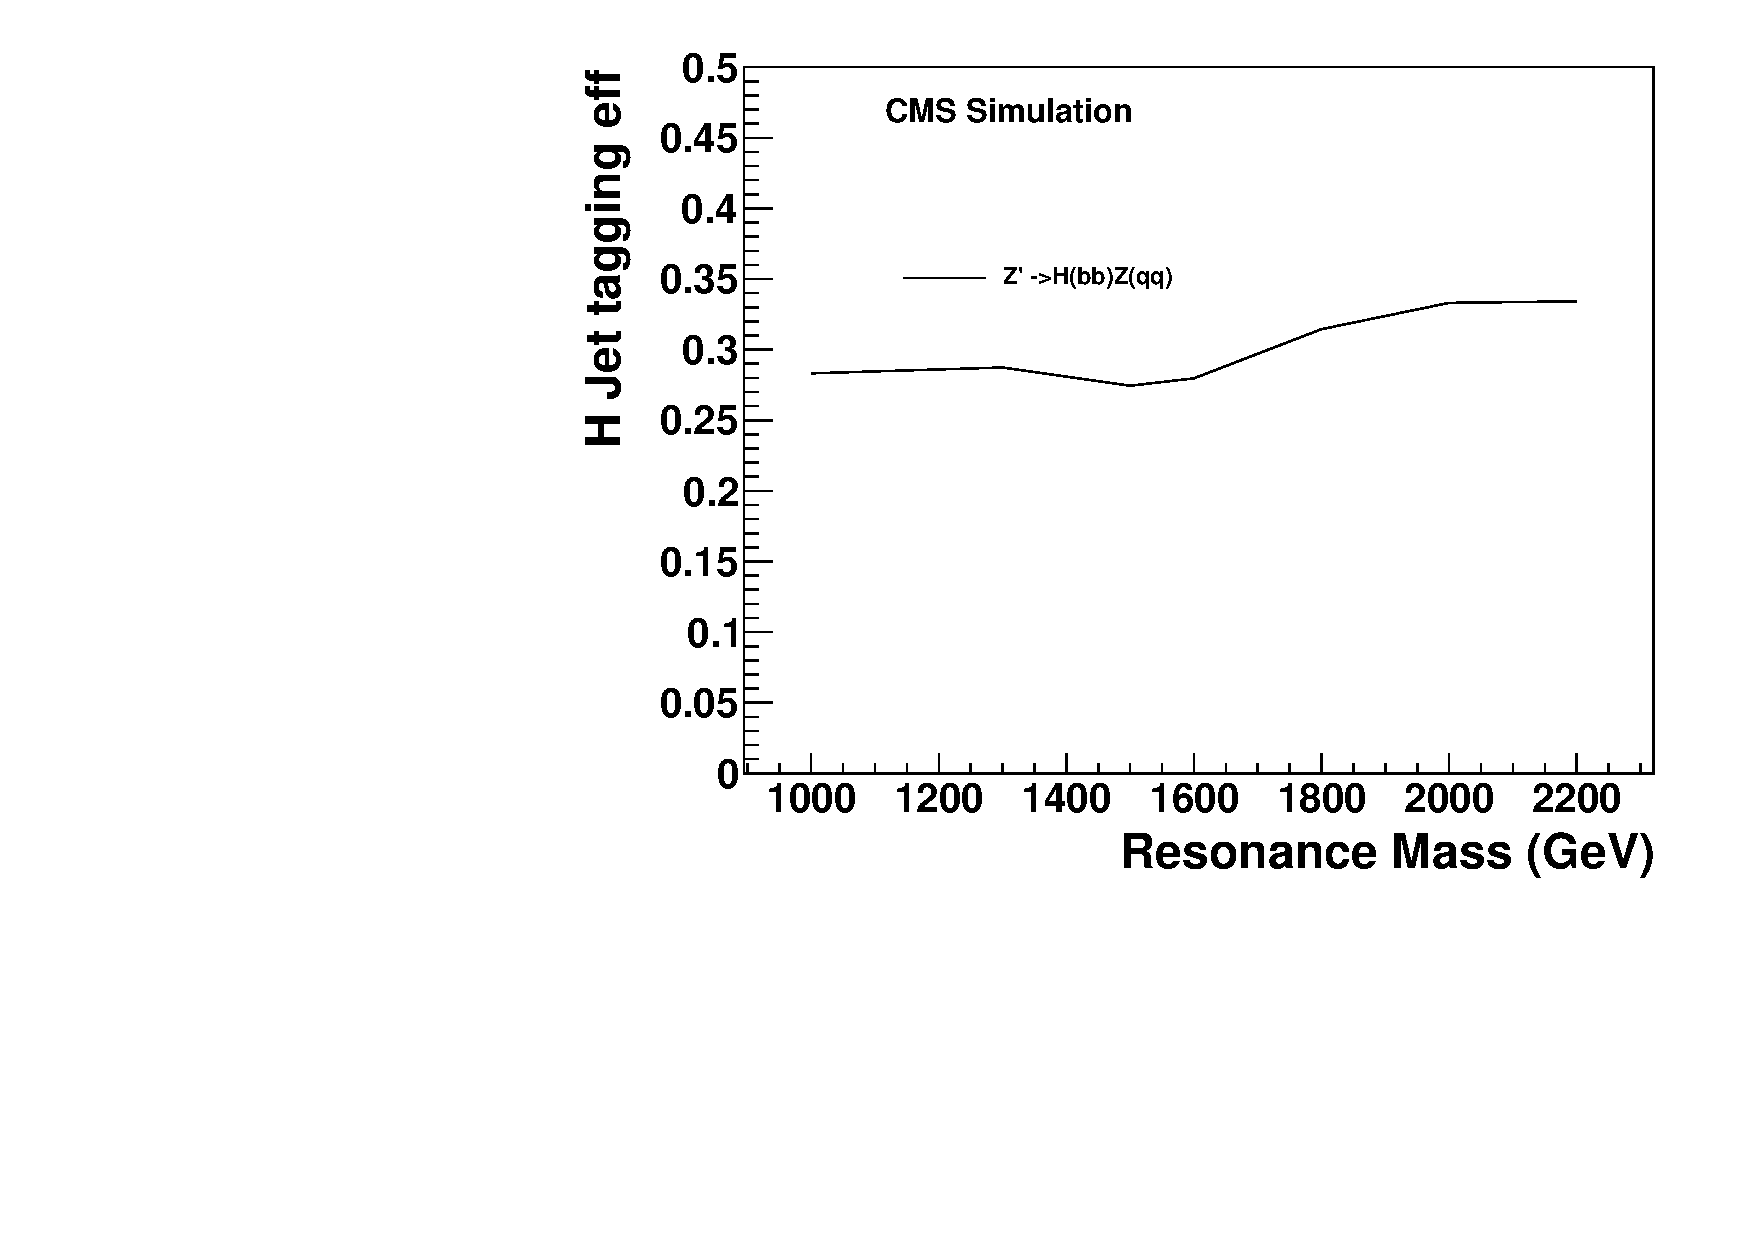
\includegraphics[width=0.49\textwidth]{EXO-14-009/HbbZqqfigs/Signal/H-taggingEff-8TeV.pdf}
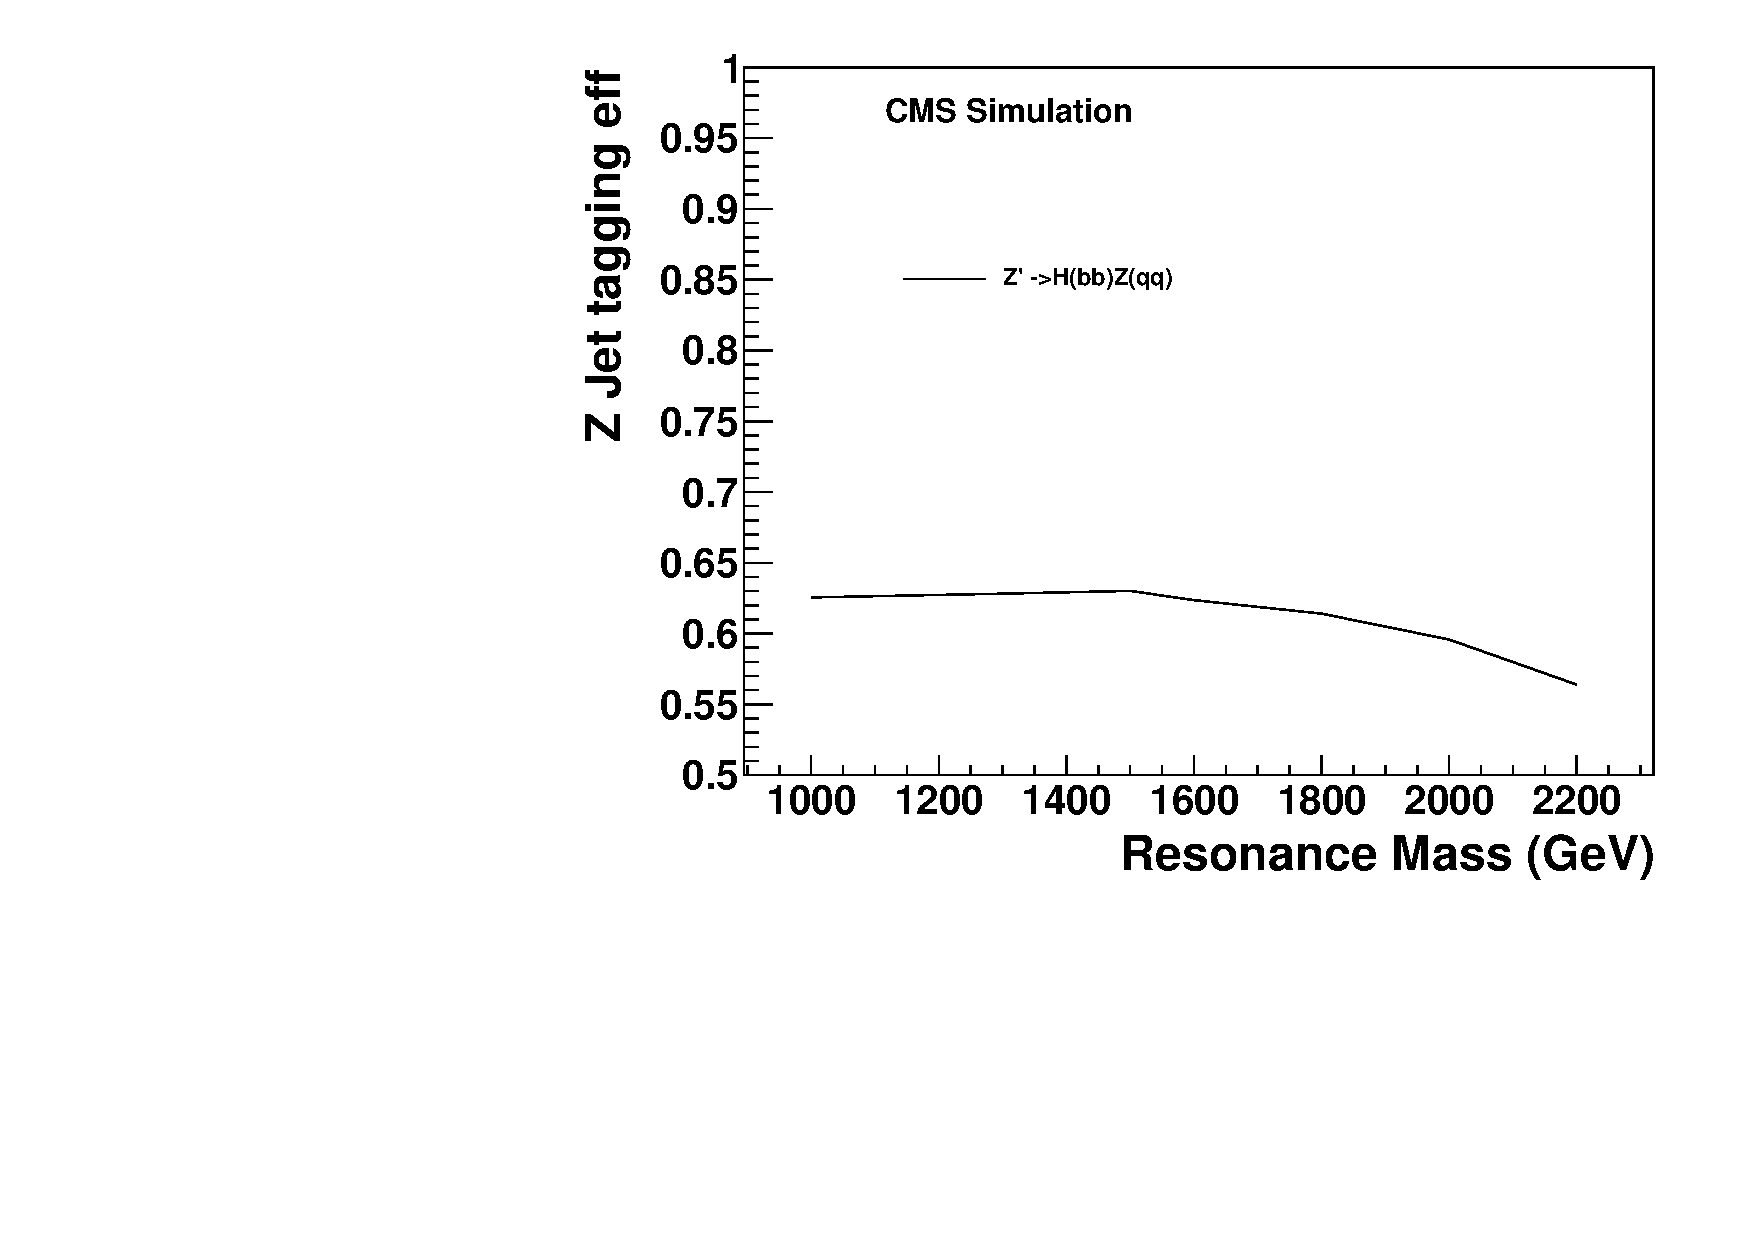
\includegraphics[width=0.49\textwidth]{EXO-14-009/HbbZqqfigs/Signal/Z-taggingEff-8TeV.pdf}
%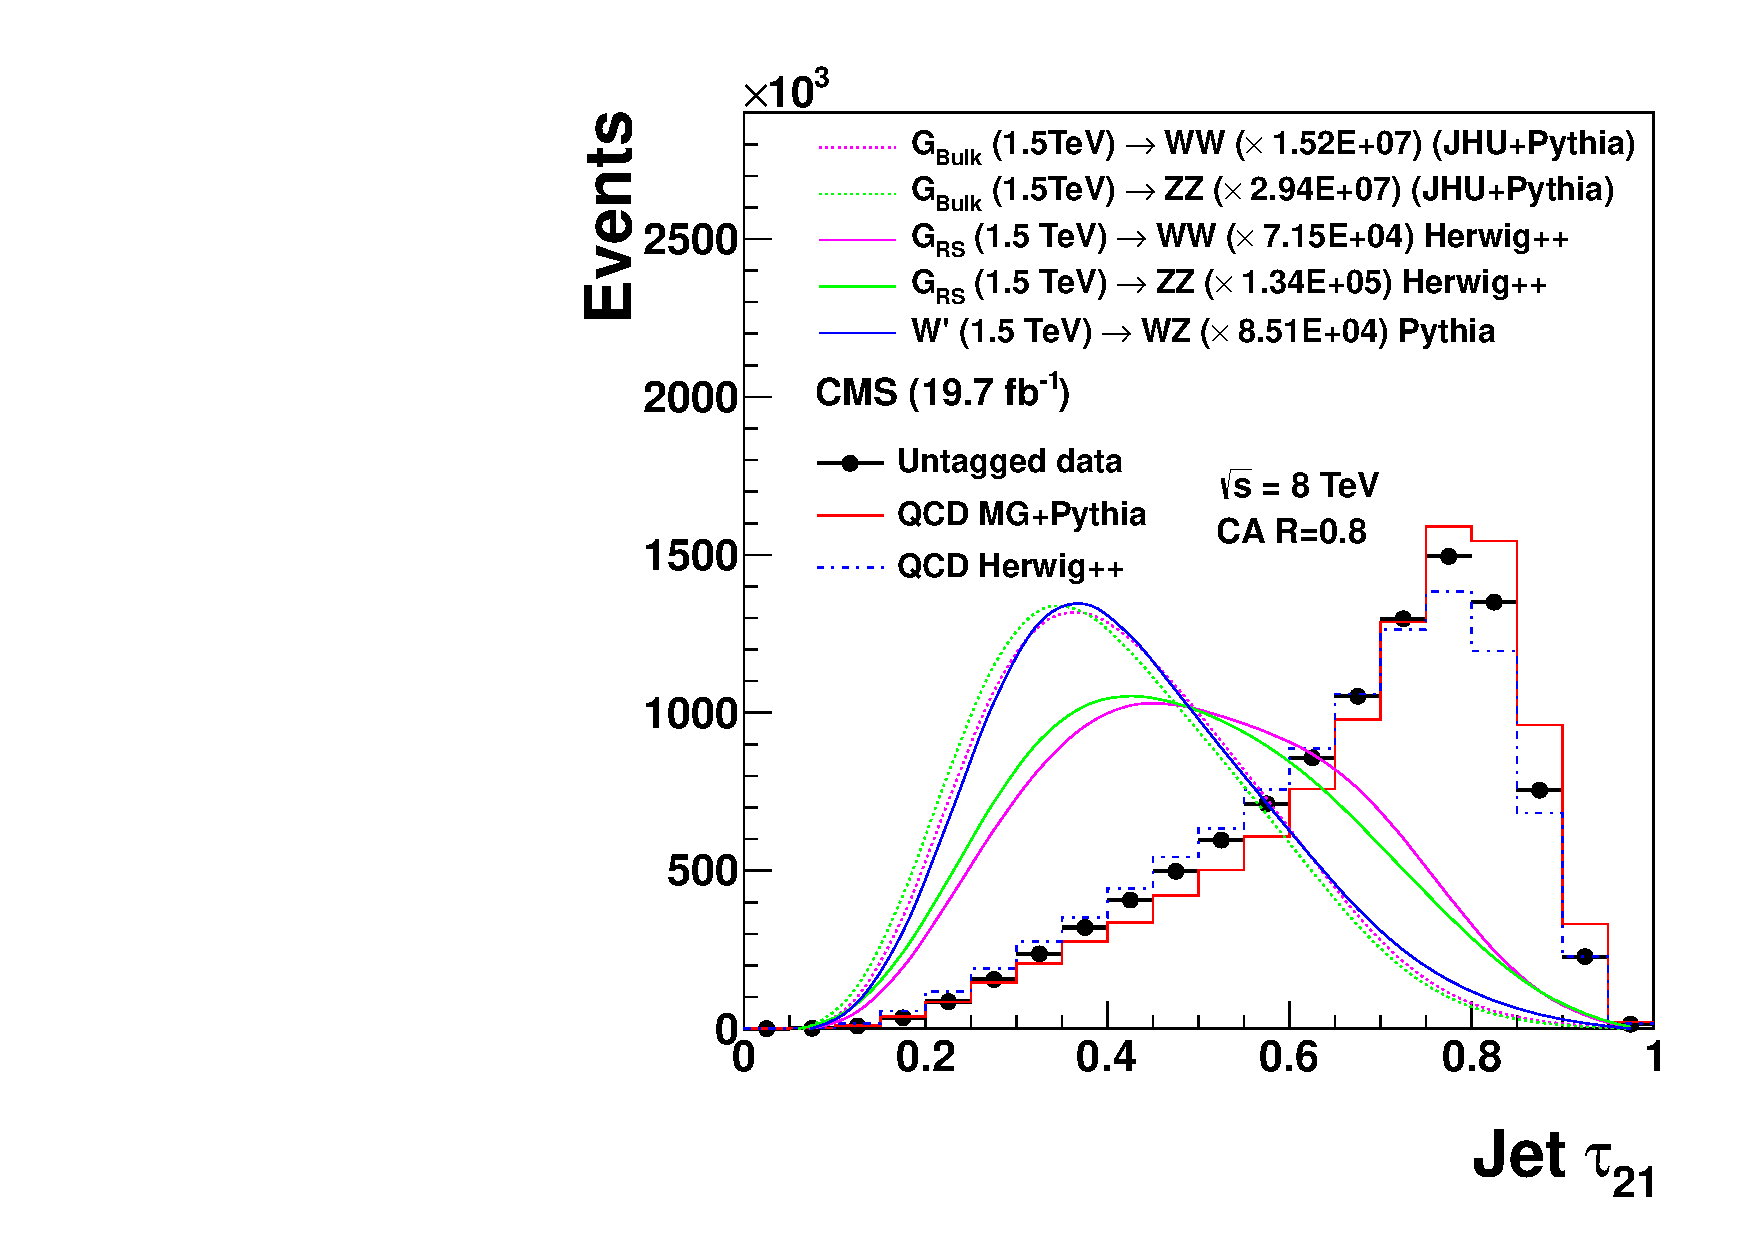
\includegraphics[width=0.49\textwidth]{figs/signal-acc-eff/signal-data-qcd-Jet-Tau21.pdf}
\end{center}
\caption{
  Higgs jets and Z jets tagging efficiencies in signal MC simulation.
  Left: $\Hbb$. Right: $\Zqq$.  The total event efficiency is a product
  of the two, resulting in a relatively flat efficiency for reconstructing
  $X \to HV$.
}
\label{fig:HEff}
\end{figure}


In the $\Hbb$ channel, the $\Hbb$ tagging efficienc start rising 
after $\sim 1.6$~\TeVcc. The reason is explained as follows.  
For the resonance masses above $1.6$~\TeVcc, the Higgs
jets are sufficiently boosted that the $\Delta R$ between the two b
subjets is $\le 0.3$. When $\Delta R \leq 0.3$, we are switching from 2 subjets
b tagging to CSV loose fat jet b tagging.  This causes the rising tagging efficiency. 

Since the CSV tagging uses the cone of $0.3$ to
associate the candidate tracks to the jet, when the two subjets are at
angular distance of $0.6$, they begin sharing tracks. 
This effect becomes important for $\Delta R \le 0.3\sim0.4$.  For this
reason, when the subjets are closer than $0.3$, following the BTV POG
recommendation, we switch to using the CSV b tagging decision for the
fat jet. (We use CSVL, the loose operating point.)

Note that if for the fat jet b tagging CSVM operating point is used,
the $\Hbb$ tagging efficiency is smooth, as shown in
Fig.~\ref{fig:fatCSVM}.  For the \HbbZqq\ analysis, we have compared
the limits of these two different fat jet b tagging methods (CSVL 
{\it vs.} CSVM), Unsurprisingly, we have found that using the
more-efficient CSVL b tagging results in better expected limits in
this background-poor region than using the CSVM b tagging operating
point. (The details of this study are given in the Appendix.)

%{\bf TO-DO: ADD CSVM limit plots to the Appendix for this, and reference it here. }


\begin{figure}[htb]
\begin{center}
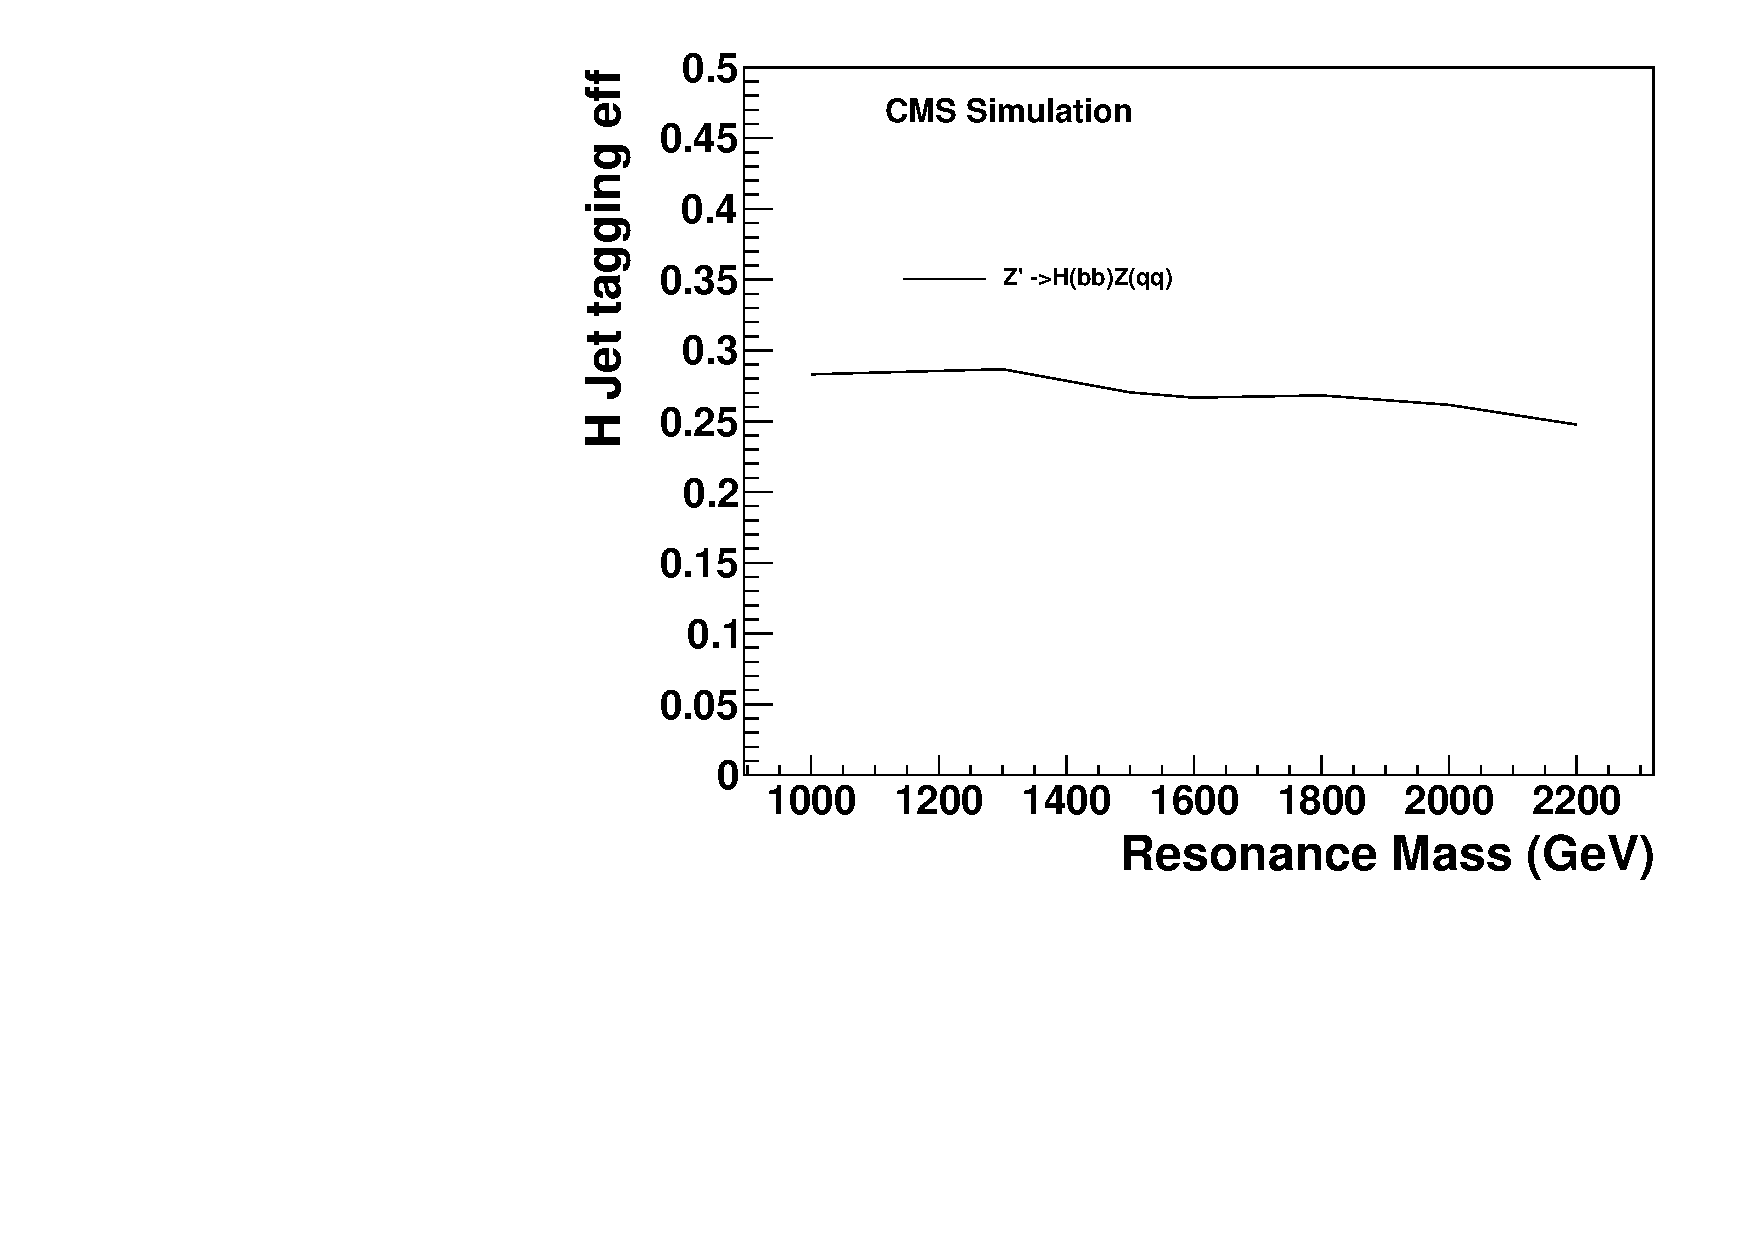
\includegraphics[width=0.60\textwidth]{EXO-14-009/HbbZqqfigs/Signal/H-taggingEff-8TeV-CSVM.pdf}
\end{center}
\caption{
  Higgs tagging efficiency in signal MC, for $\Hbb$ channel.  
  Changing fat jet b tagging to CSVM instead of CSVL. 
}
\label{fig:fatCSVM}
\end{figure}

\clearpage

\subsection{Signal acceptance and total efficiency for \HbbZqq\ channel}

Signal acceptance is defined as the number of signal events pass all
the kinematic event selection (that is, without the two jet-tagging
algorithms) divided by the number of generated events.  The signal
acceptance for \HbbZqq\ channel is shown on Fig.~\ref{fig:Acc}.

\begin{figure}[htb]
\begin{center}
\includegraphics[width=0.49\textwidth]{EXO-14-009/HbbZqqfigs/Signal/HbbZqq-signal-acc-8TeV.pdf}
%\includegraphics[width=0.49\textwidth]{HqqqqZqqfigs/Signal/HqqqqZqq-signal-acc-8TeV.pdf}
\end{center}
\caption{
Acceptance in \HbbZqq\ signal.
}
\label{fig:Acc}
\end{figure}

The combined tagging rate of H and Z tagging, is defined as the number of 
events pass the HZ-tagging dvided by the number of events after events
selection, which is shown in Fig.~\ref{fig:HbbZqqOverallEff} for \HbbZqq\ 
tagging. 

\begin{figure}[htb]
\begin{center}
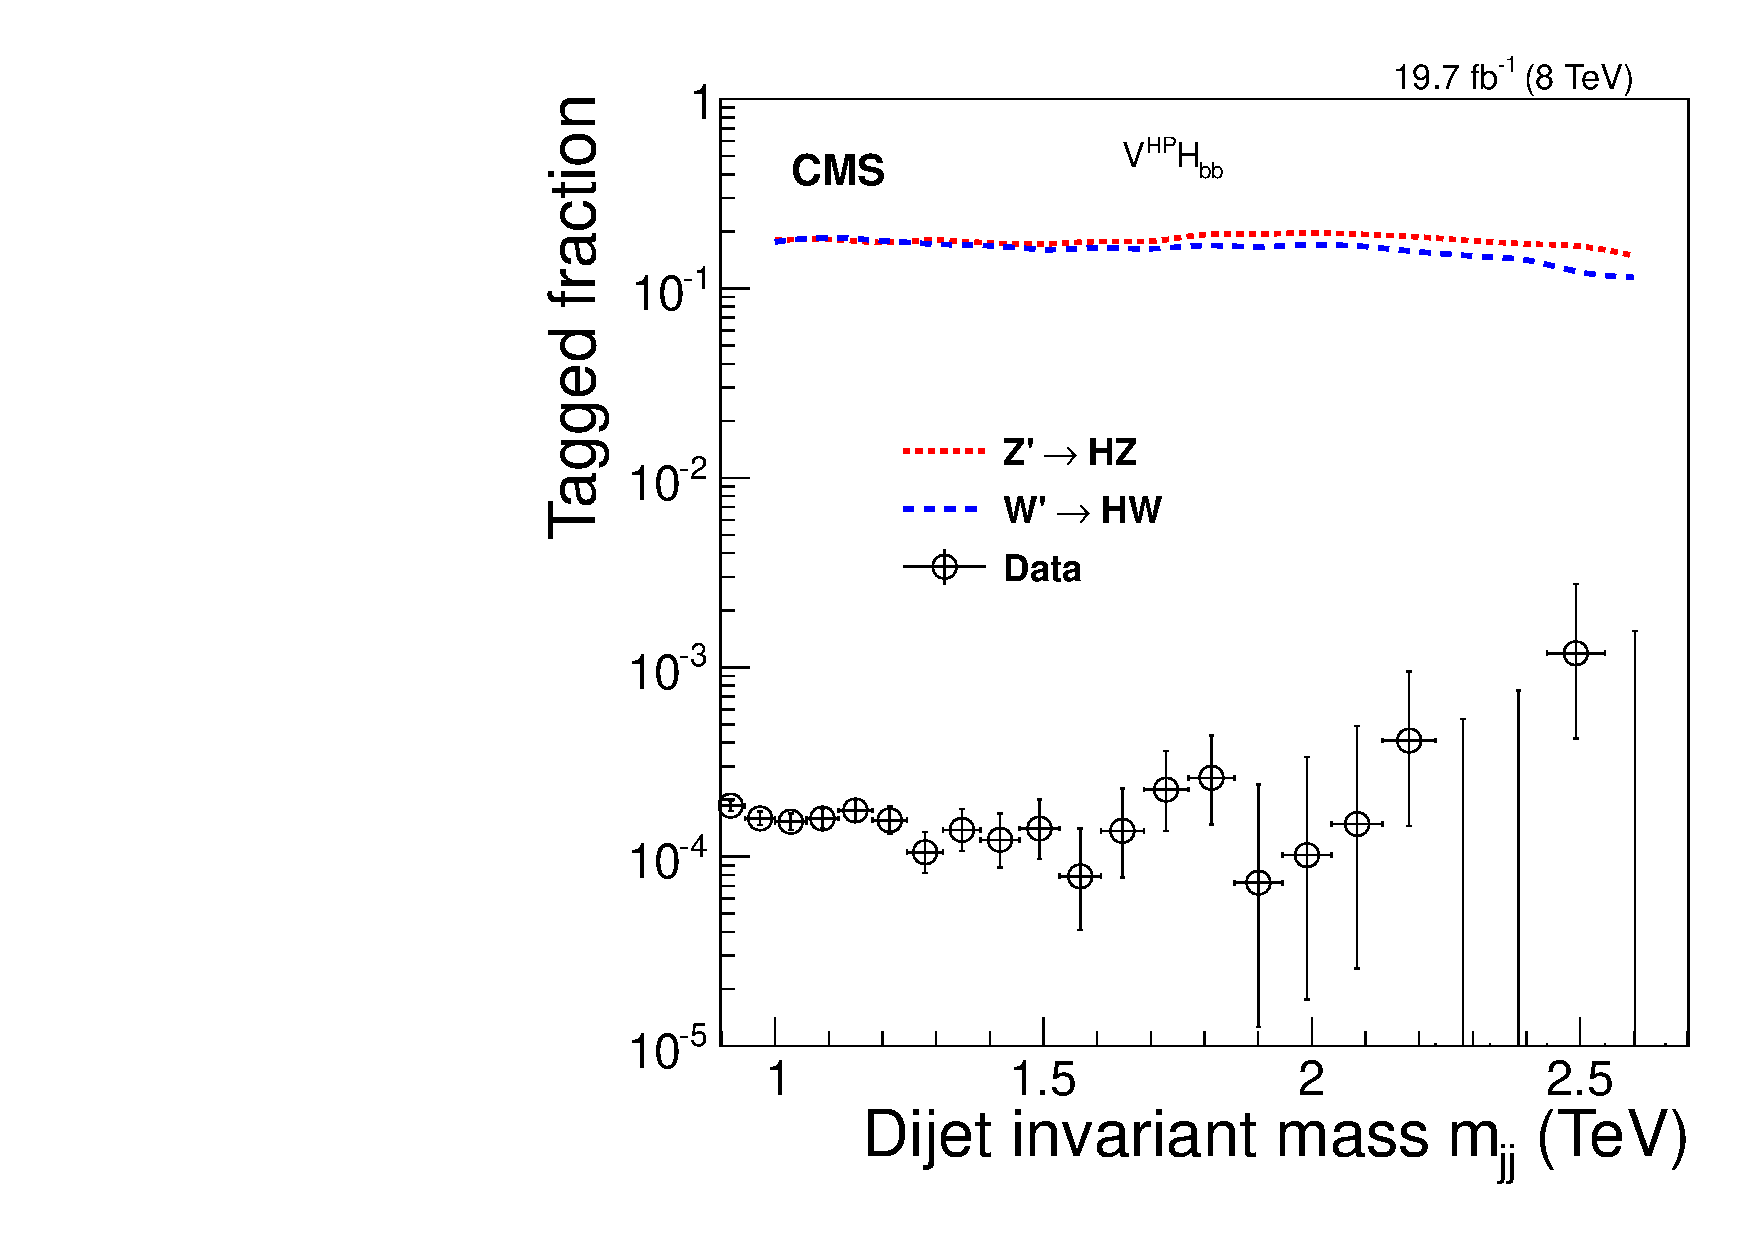
\includegraphics[width=0.49\textwidth]{EXO-14-009/HbbZqqfigs/Signal/HbbVqq-signal-taggingEff-8TeV.pdf}
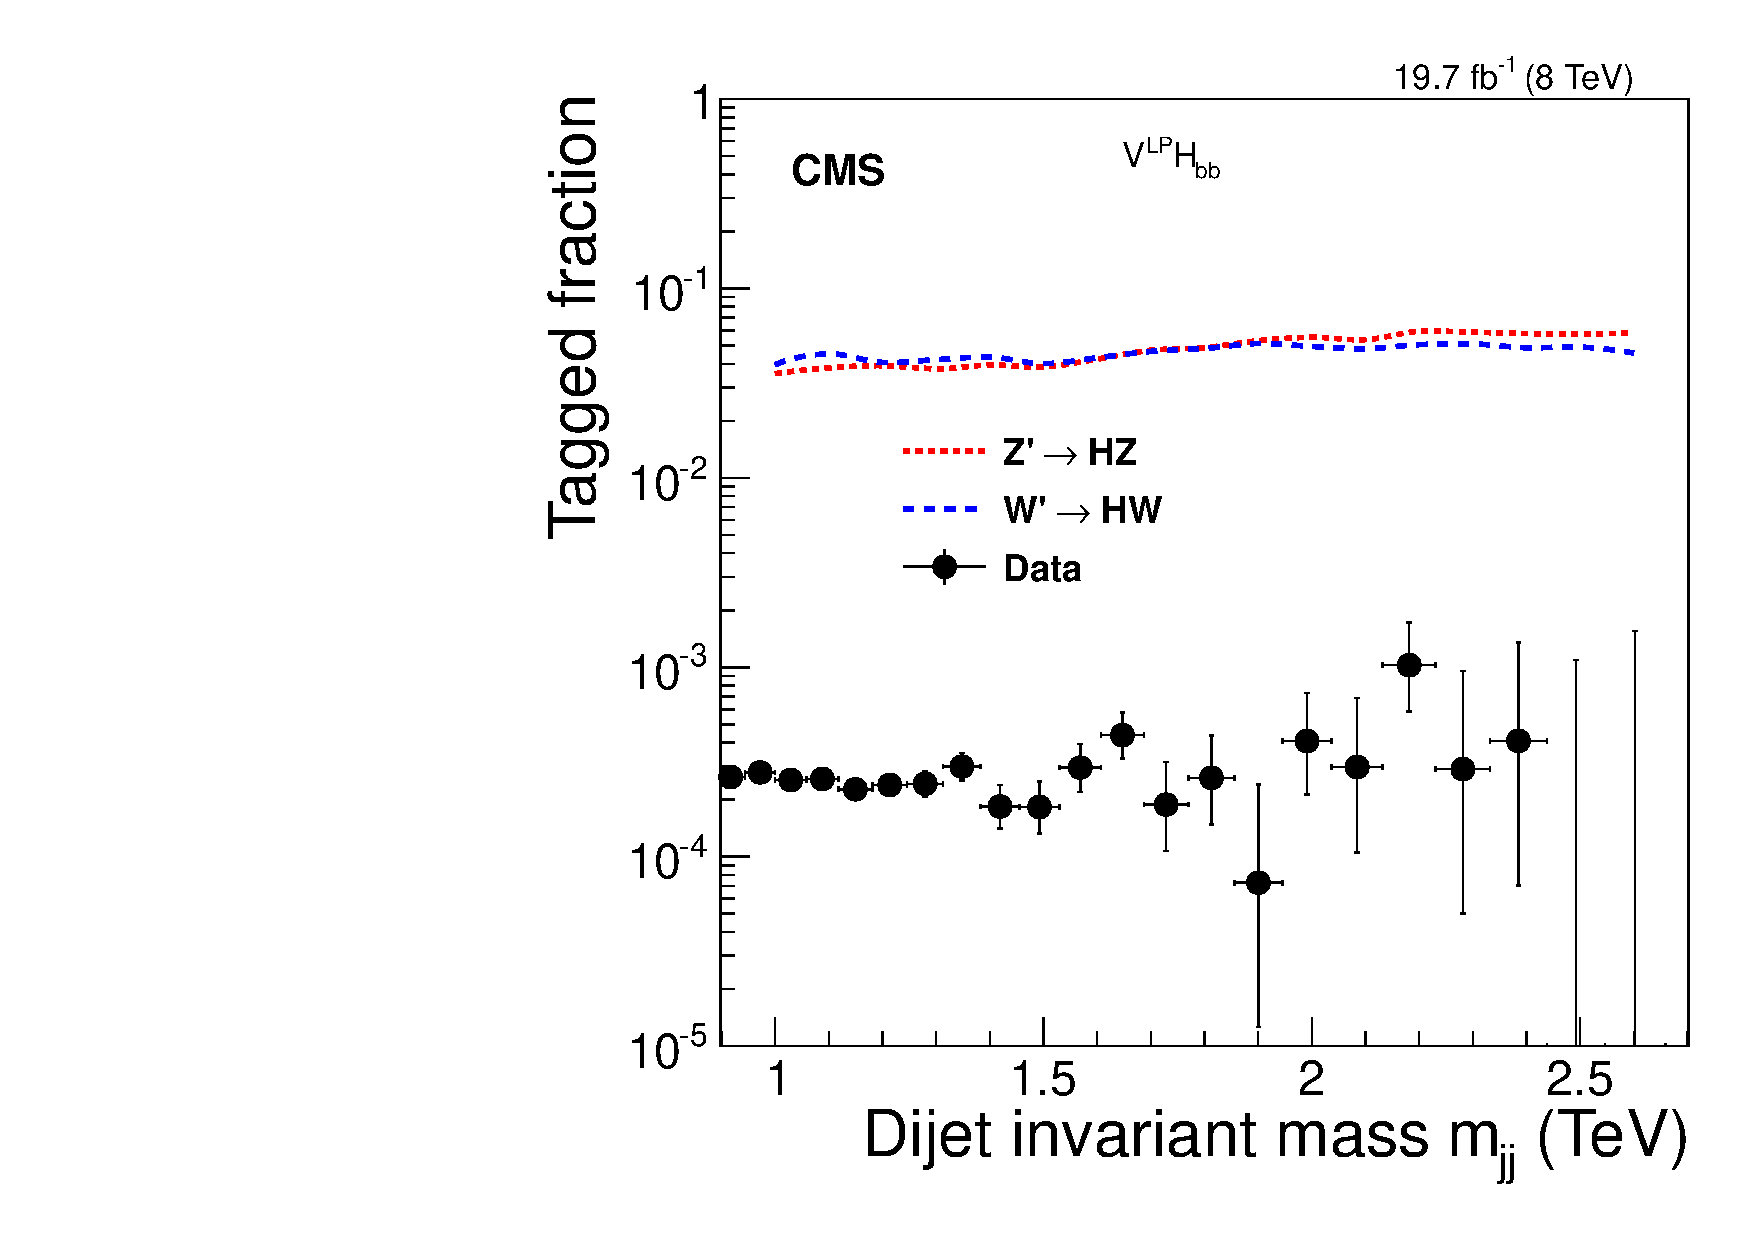
\includegraphics[width=0.49\textwidth]{EXO-14-009/HbbZqqfigs/Signal/HbbVqq-signal-taggingEff-LowV-8TeV.pdf}
%\includegraphics[width=0.49\textwidth]{HqqqqZqqfigs/Signal/HqqqqZqq-signal-acc-8TeV.pdf}
\end{center}
\caption{
Tagging rates in \HbbZqq\ and \HbbWqq\ signal channels and data. Horizontal bars
in data indicates variable binning size.
}
\label{fig:HbbZqqOverallEff}
\end{figure}

%The signal shapes are shown in Fig.\ref{fig:HbbZqqShape}
%\begin{figure}[htb]
%\begin{center}
%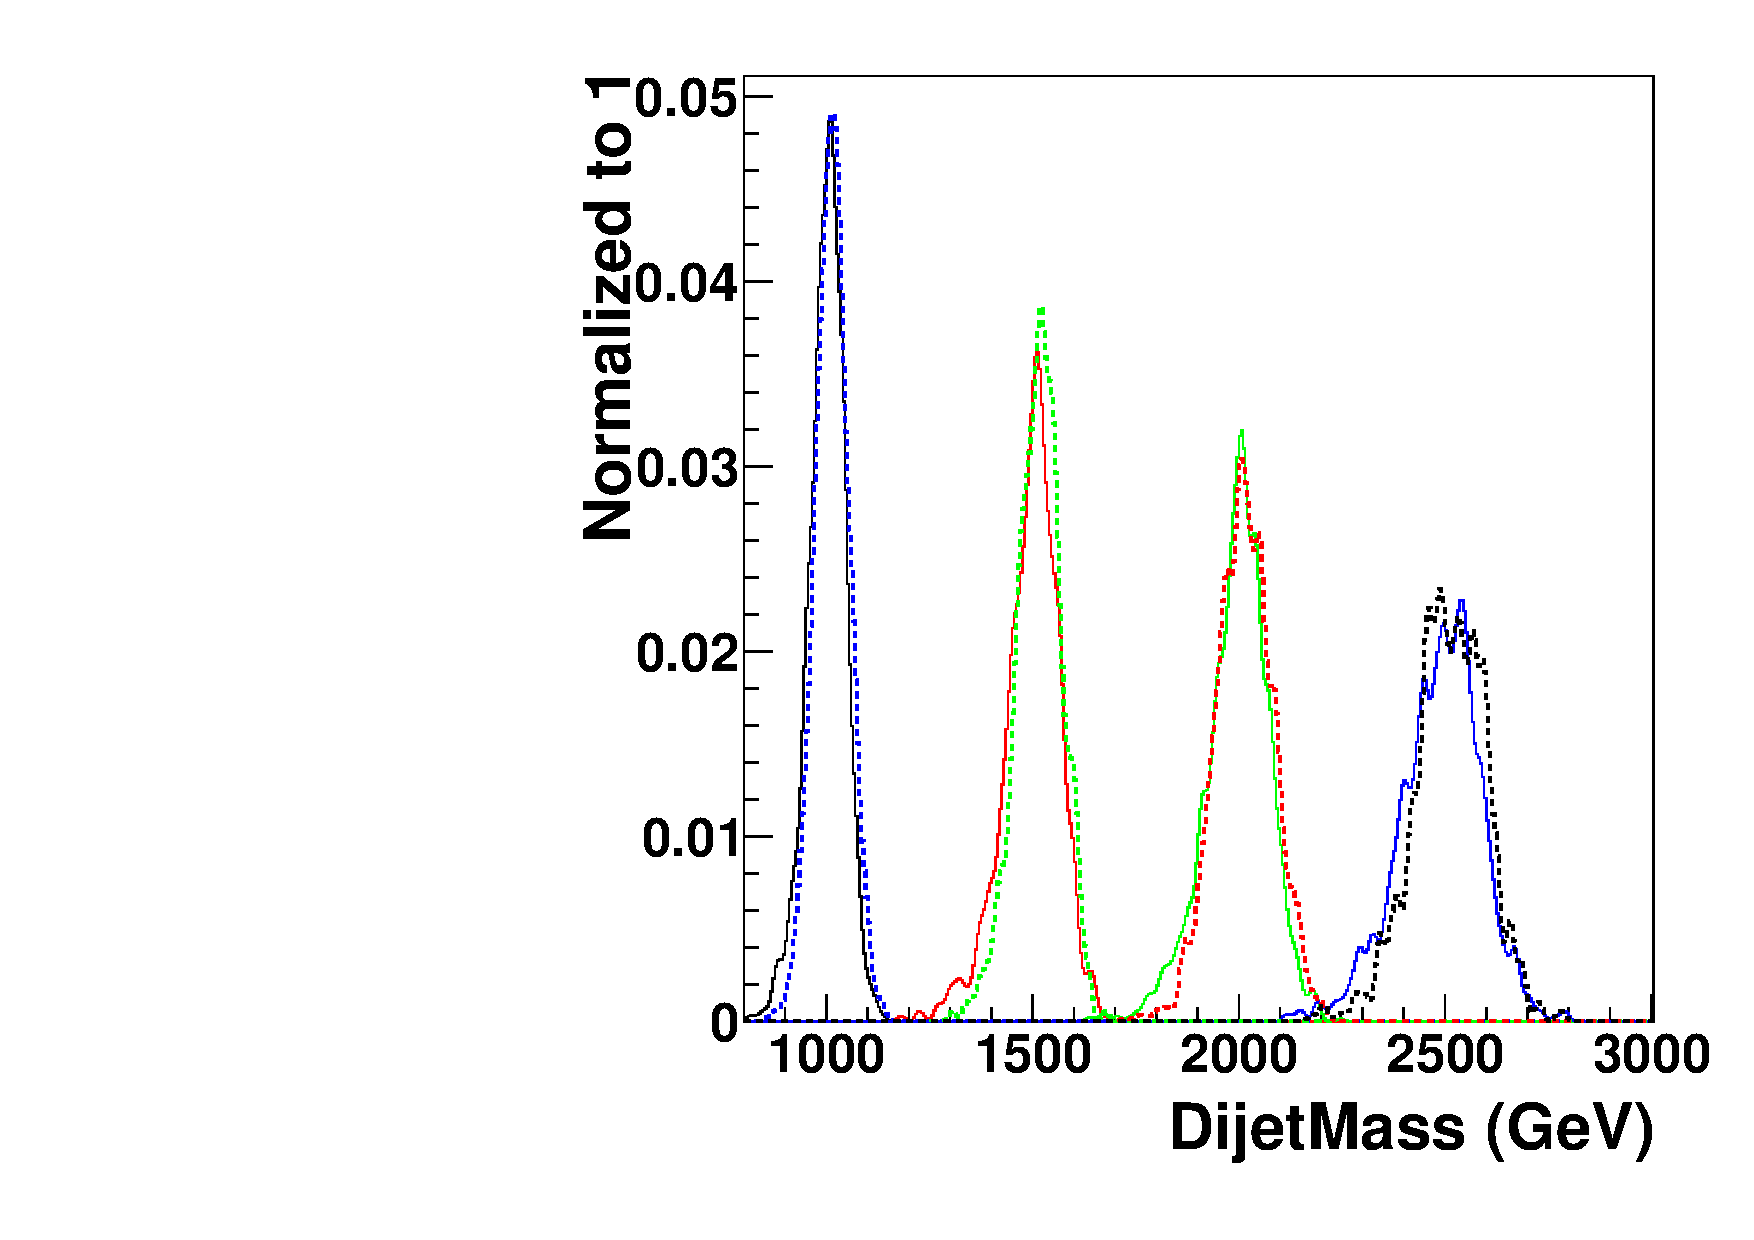
\includegraphics[width=0.69\textwidth]{HbbZqqfigs/Signal/shapeHbbZqq.pdf}
%\end{center}
%\caption{Signal shapes for Z' and W' signals at 1.0, 1.5, 2.0 and 2.5 TeV resonance. 
% Z' are shown in solid lines.
%W' are shown in dashed lines.
%}
%\label{fig:HbbZqqShape}
%\end{figure}



%{\bf TO-DO: add the signal shapes.}

%{\bf TO-DO: add distributions of $\eta$, $\Delta\eta$.}

\clearpage





\subsection{Tagging efficiency for $\Hww$ jets}


The tagging efficiency for $\Hww$ jets, as a fraction of getJets that
passes the selection, is shown in Fig.~\ref{fig:HwwEff}.
\begin{figure}[htb]
\begin{center}
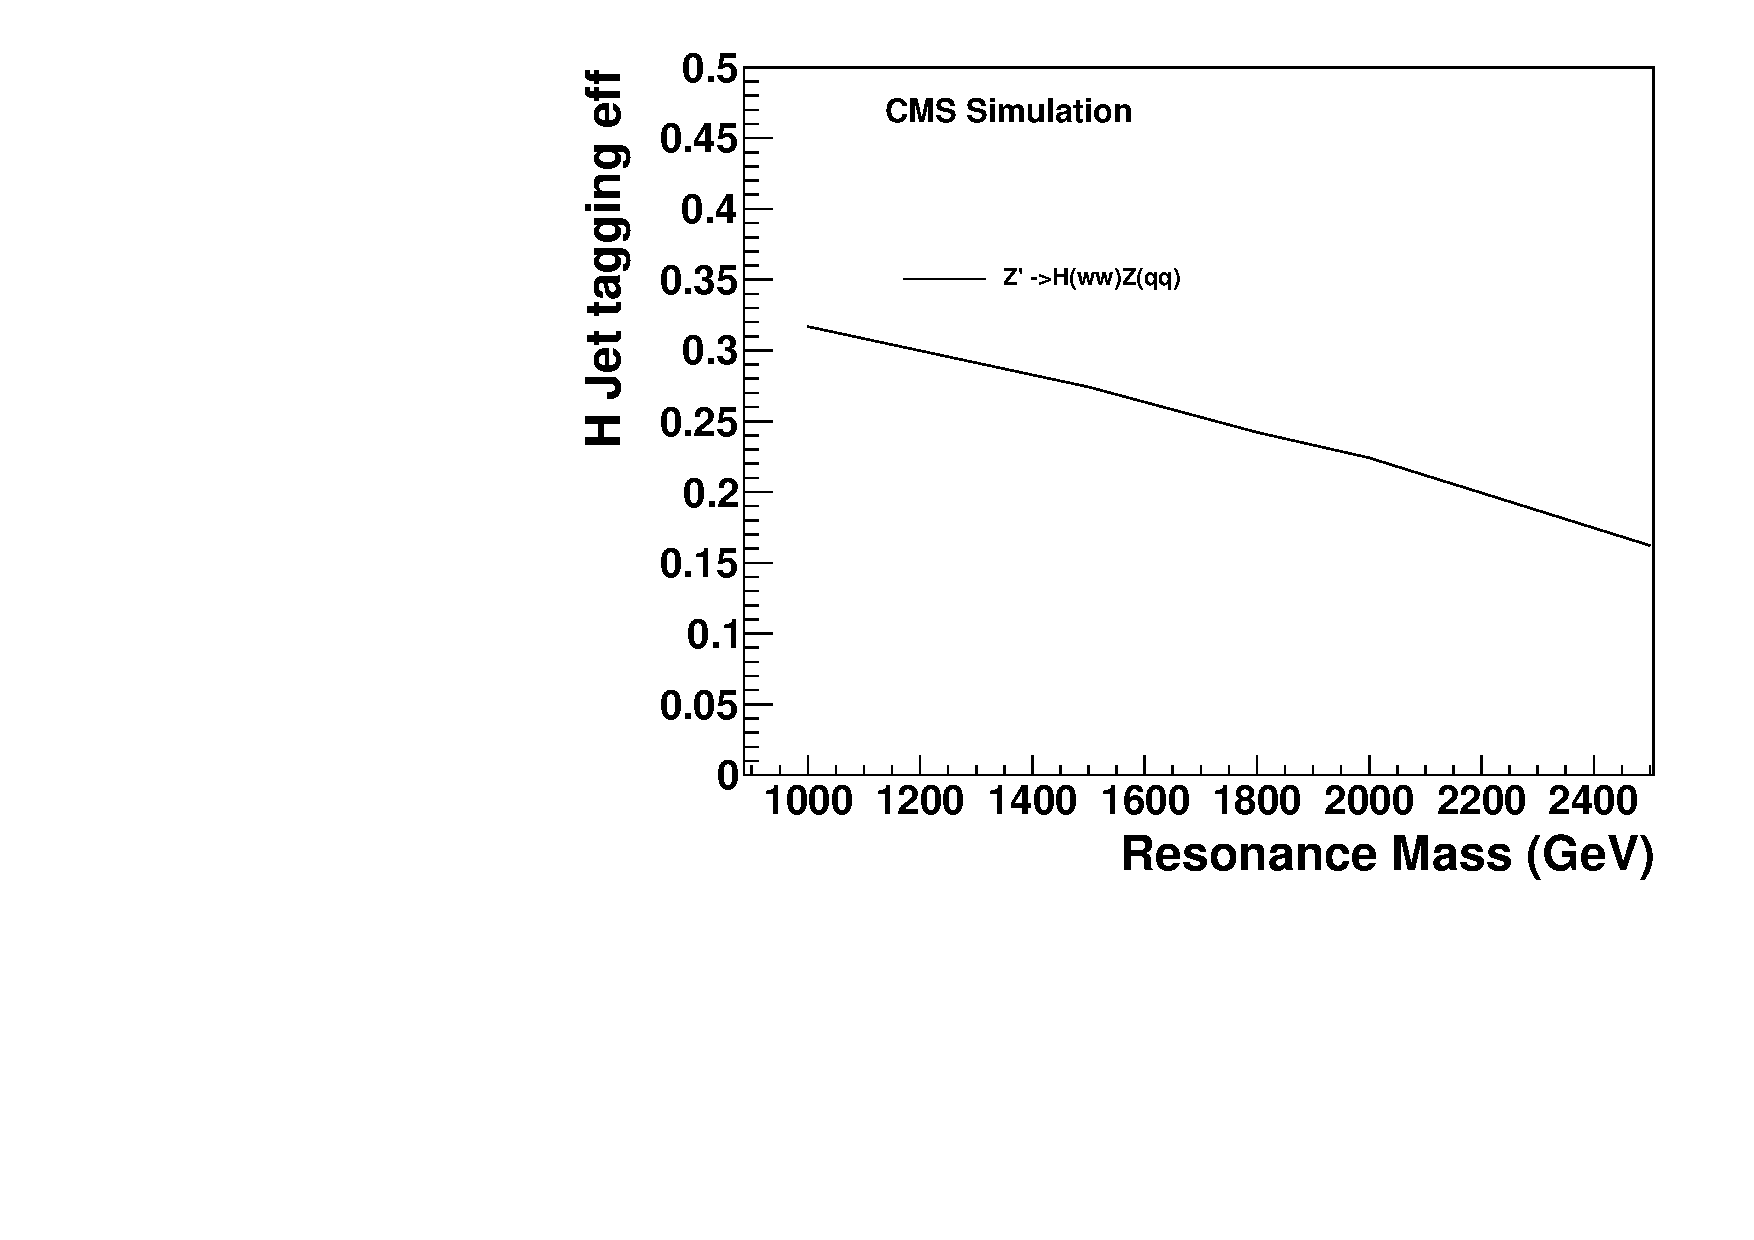
\includegraphics[width=0.49\textwidth]{EXO-14-009/HqqqqZqqfigs/Signal/H-taggingEff-8TeV.pdf}
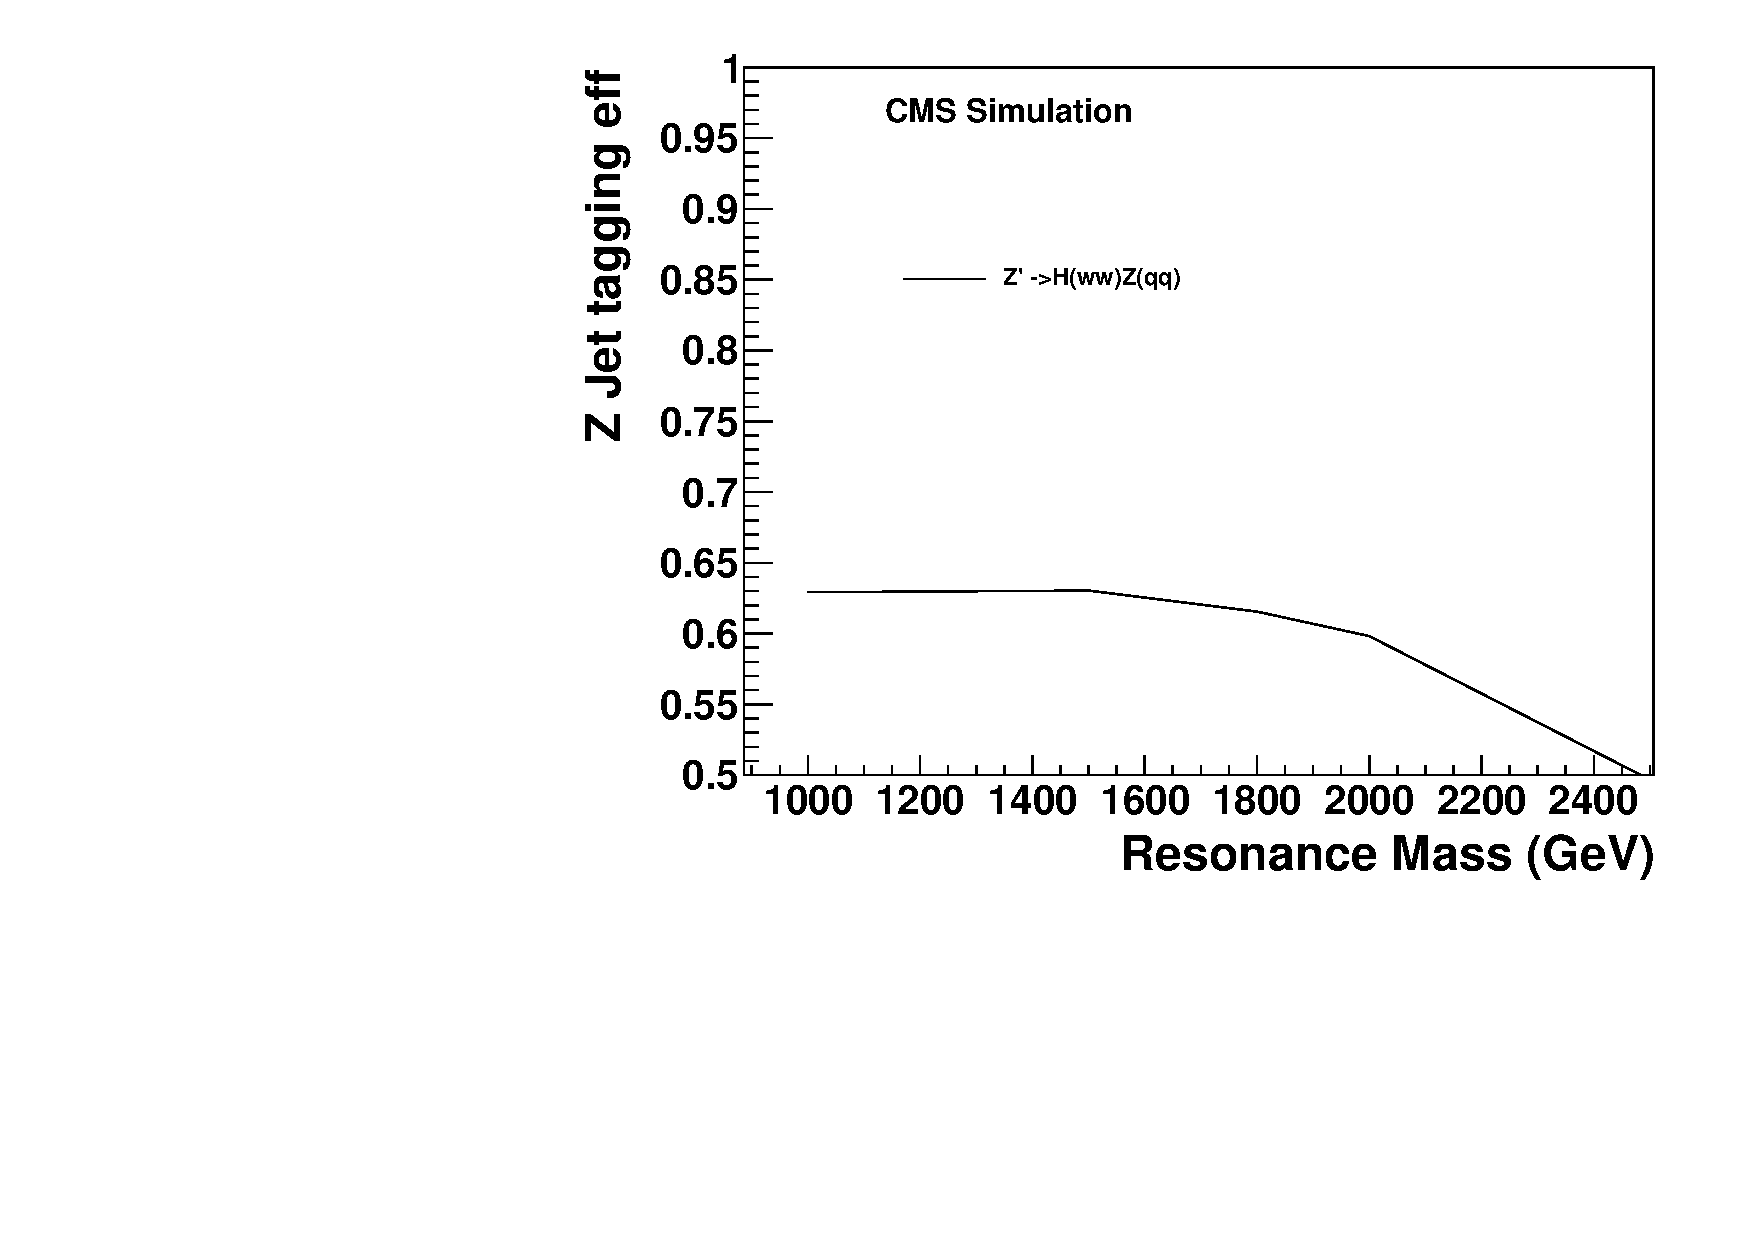
\includegraphics[width=0.49\textwidth]{EXO-14-009/HqqqqZqqfigs/Signal/Z-taggingEff-8TeV.pdf}
\end{center}
\caption{
  Higgs jets and Z jets tagging efficiencies in signal MC simulation.
  Left: $\Hww$. Right: $\Zqq$.  The total event efficiency is a product
  of the two, resulting in a following spectrum efficiency for reconstructing
  $X \to HV$.
}
\label{fig:HwwEff}
\end{figure}
 

In the $\Hww$ all-hadronic channel, to compensate the efficiency loss
in the high resonance mass, we also add two low purity categories, low
purity H-tagging and low purity V-tagging.  The tagging efficiency of
low purity H/V-tagging on the H/Z jets is shown on
Fig.~\ref{fig:LowPurity}.  And low purity Higgs is defined as 
$0.55 < \tau_{42} < 0.65$, pruned jet mass in $[110, 135]$~\GeVcc.  

For low purity W/Z tagging, $\tau_{21}$ must be in $[0.5, 0.75]$, 
and the pruned jet mass in the window $[70, 100]$~\GeVcc.


\begin{figure}[htb]
\begin{center}
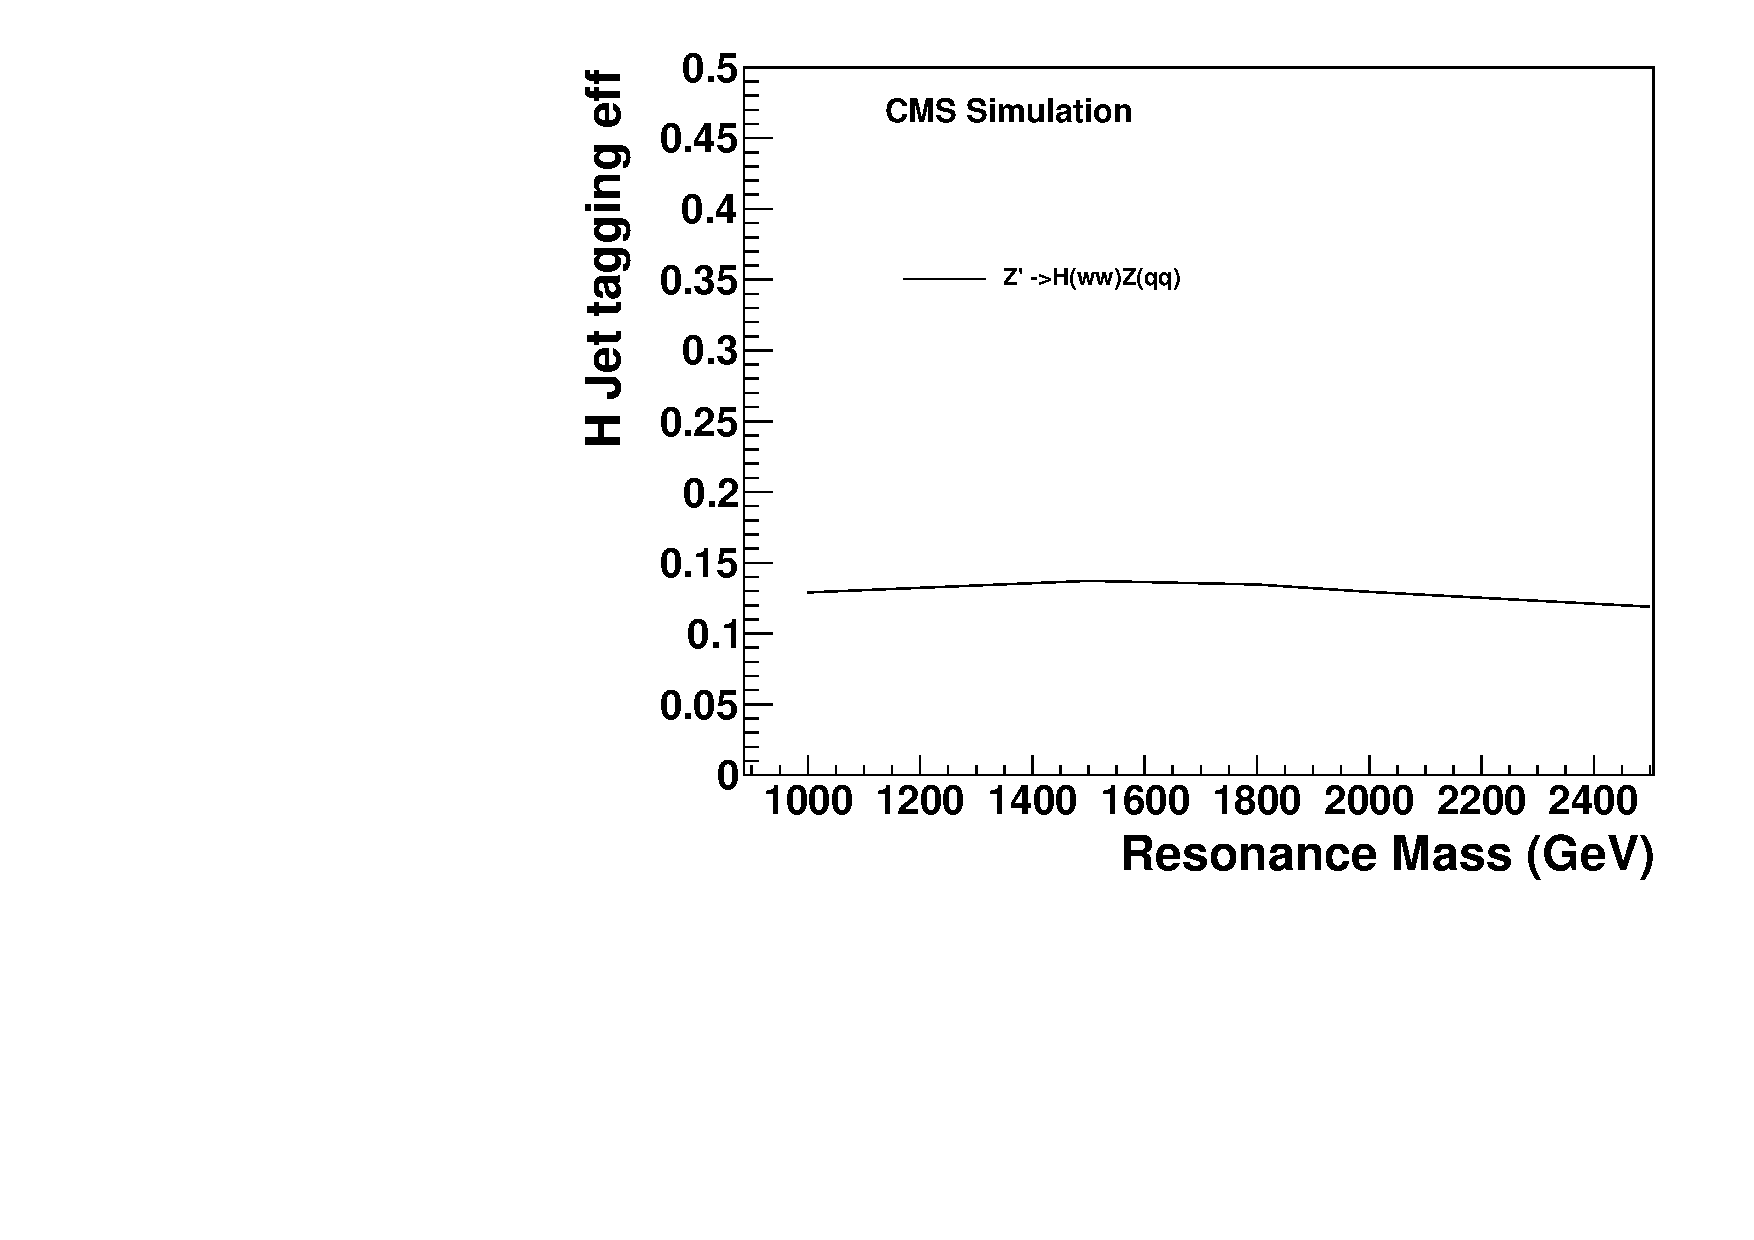
\includegraphics[width=0.49\textwidth]{EXO-14-009/HqqqqZqqfigs/Signal/H-taggingEff-8TeV-LowP.pdf}
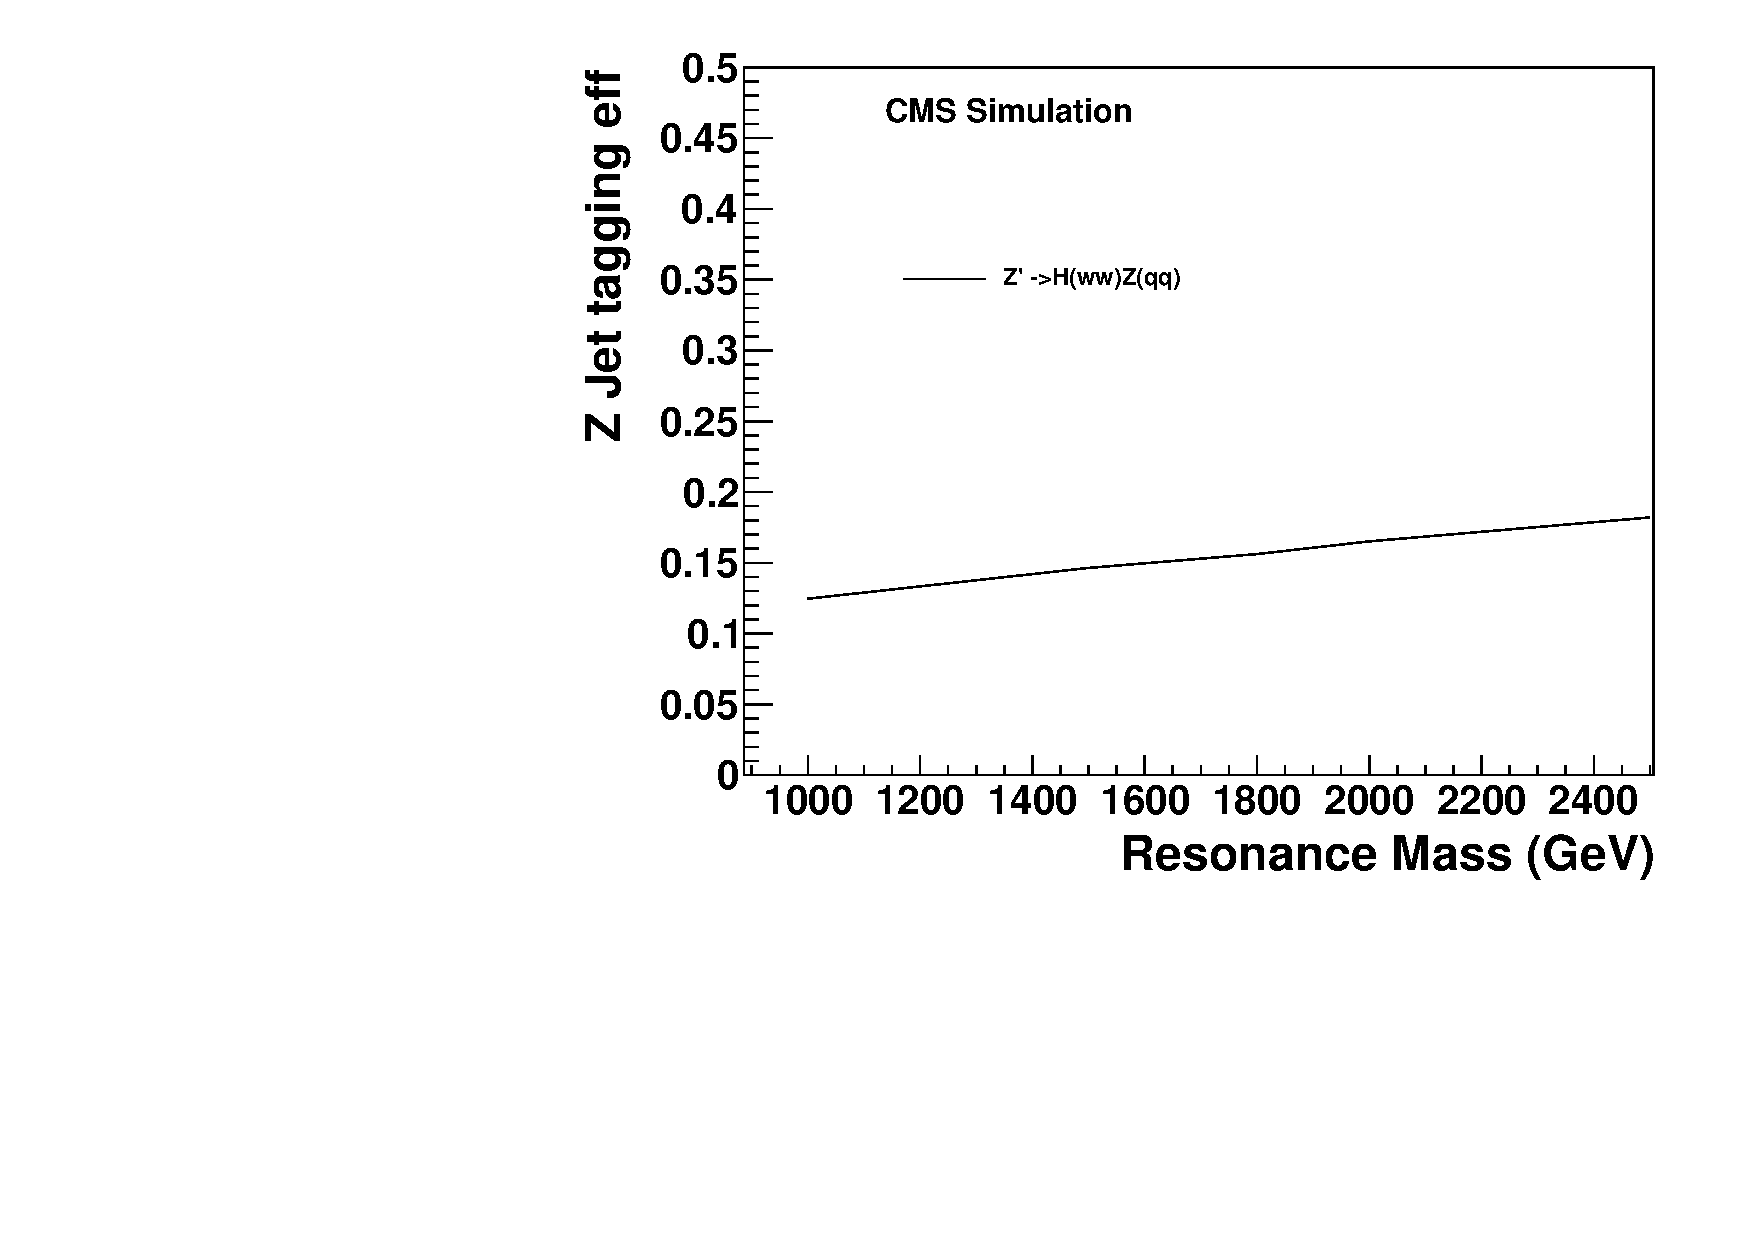
\includegraphics[width=0.49\textwidth]{EXO-14-009/HqqqqZqqfigs/Signal/Z-taggingEff-8TeV-LowP.pdf}
\end{center}
\caption{
  Lwo purity Higgs jets and Z jets tagging efficiencies in signal MC simulation.
  Left: $\Hww$. Right: $\Zqq$.  }
\label{fig:LowPurity}
\end{figure}



\subsection{Signal acceptance and total efficiency for \HwwZqq\ channel}

The acceptance of the \HwwZqq\ channel is shown on Fig.~\ref{fig:HwwAcc}

\begin{figure}[htb]
\begin{center}
%\includegraphics[width=0.49\textwidth]{HbbZqqfigs/Signal/HbbZqq-signal-acc-8TeV.pdf}
\includegraphics[width=0.49\textwidth]{EXO-14-009/HqqqqZqqfigs/Signal/HqqqqZqq-signal-acc-8TeV.pdf}
\end{center}
\caption{
Acceptance in signal. 
}
\label{fig:HwwAcc}
\end{figure}

%The overall tagging eff of \HwwZqq\ channel in signal and data are shown
The combined tagging rates of H and Z tagging, 
for \HwwZqq\ channel in signal and data are shown on Fig.~\ref{fig:HwwEffAll} .
%and the tagging eff of \HwwZqq\ channel
%are shown on Fig.~\ref{fig:HwwEff}

\begin{figure}[ht!b]
\begin{center}
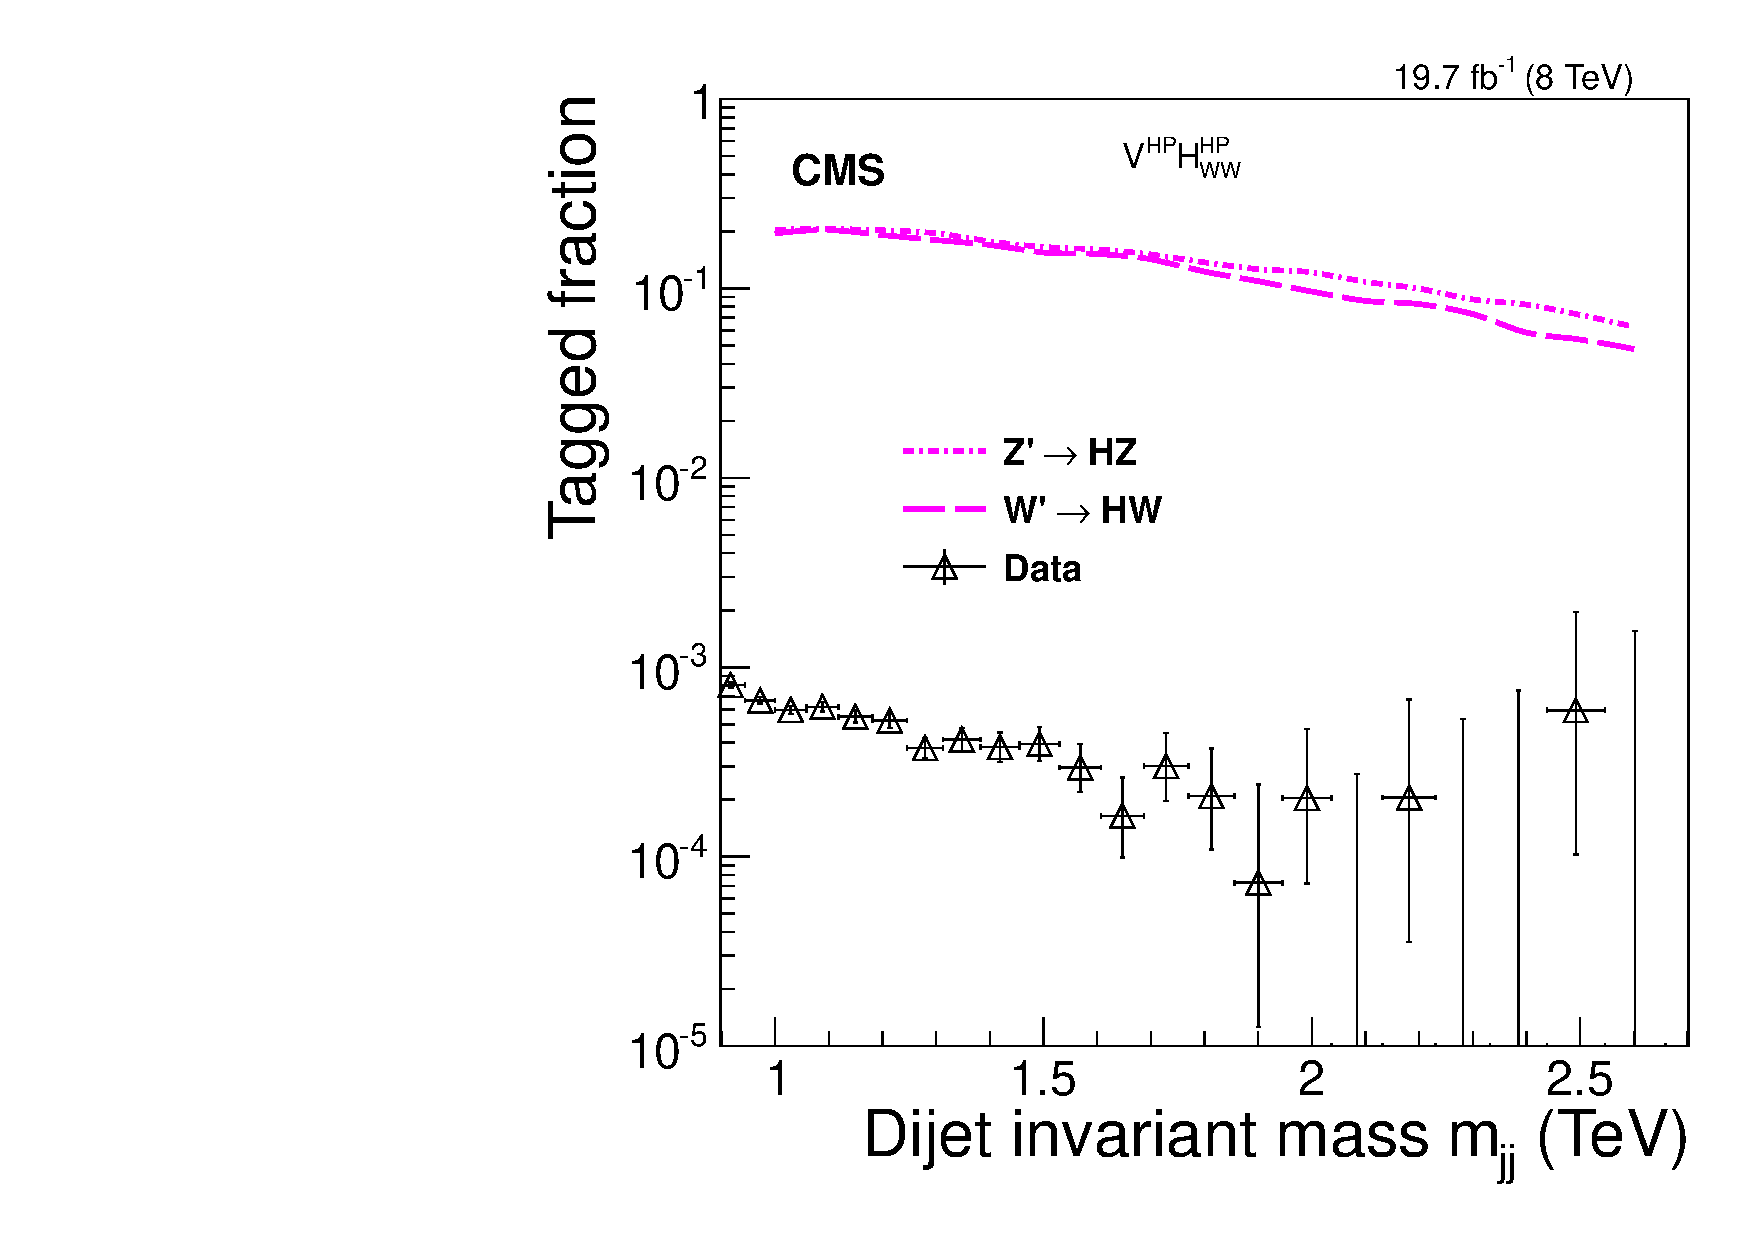
\includegraphics[width=0.70\textwidth]{EXO-14-009/HqqqqZqqfigs/Signal/HwwVqq-signal-taggingEff-8TeV.pdf}
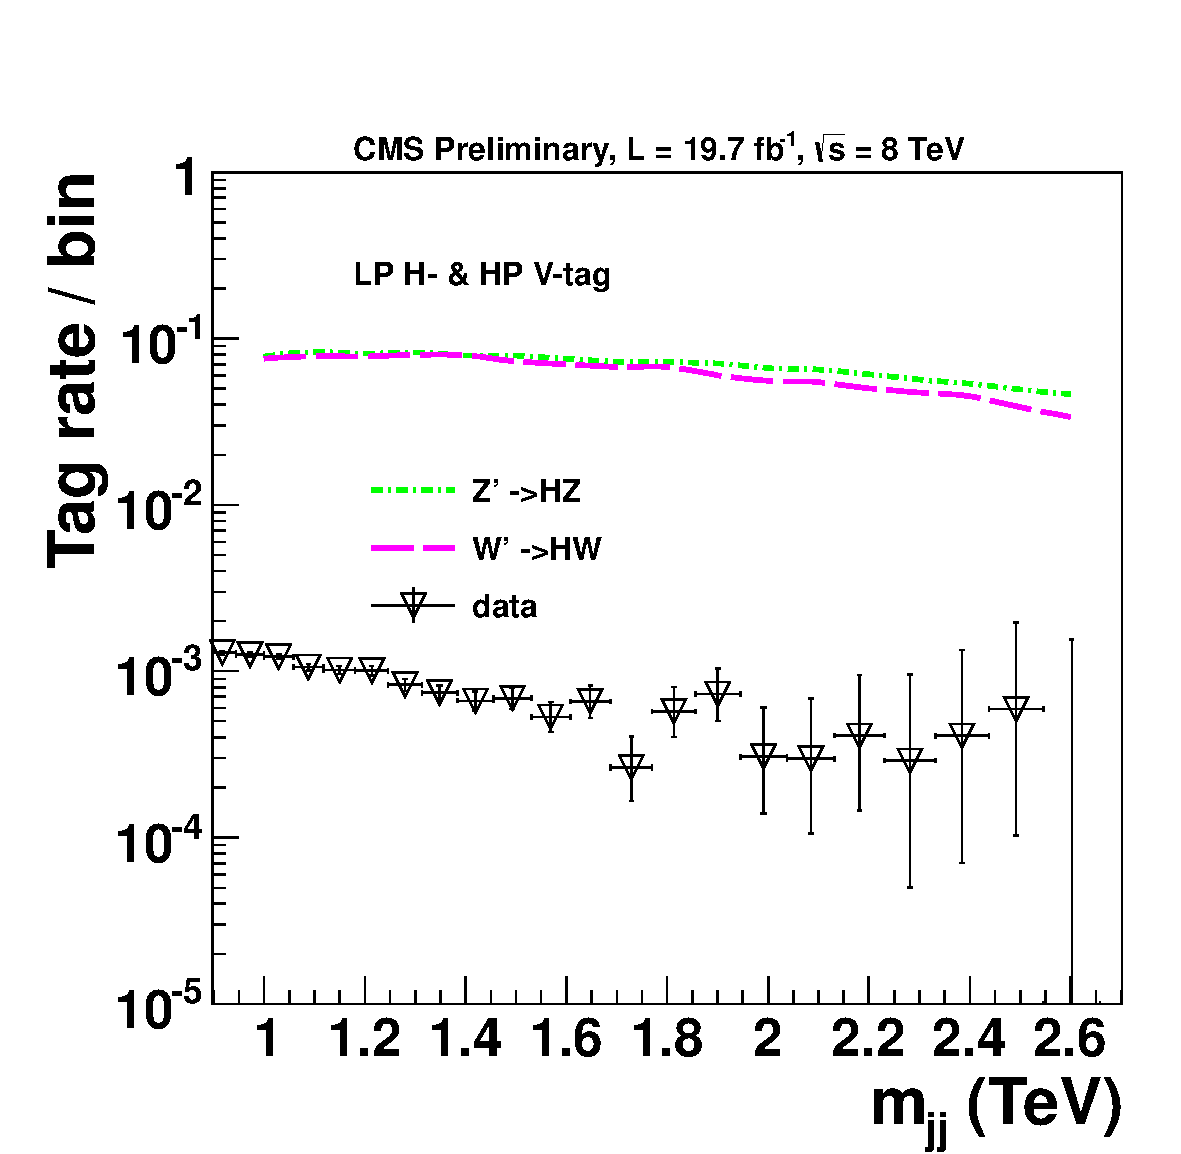
\includegraphics[width=0.49\textwidth]{EXO-14-009/HqqqqZqqfigs/Signal/HwwVqq-signal-taggingEff-LowH-8TeV.pdf}
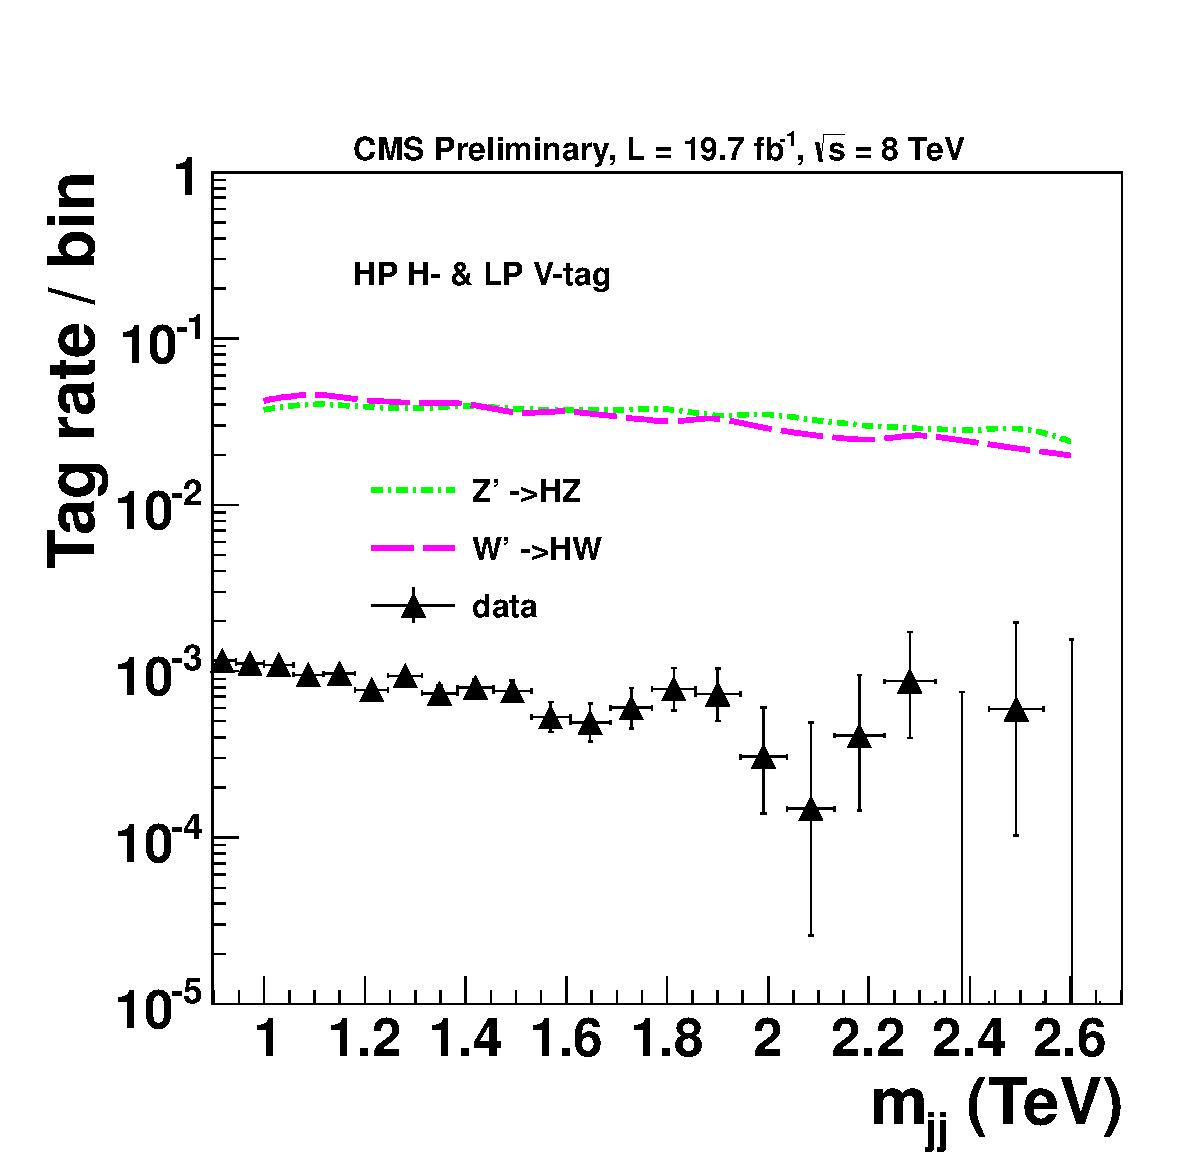
\includegraphics[width=0.49\textwidth]{EXO-14-009/HqqqqZqqfigs/Signal/HwwVqq-signal-taggingEff-LowV-8TeV.pdf}
\end{center}
\caption{
Tagging rates in \HwwZqq\ and \HwwWqq\ signal channels and data.
Horizontal bars
in data indicates variable bins.}
\label{fig:HwwEffAll}
\end{figure}

The signal shapes are shown in Fig.~\ref{fig:HbbZqqShape} 
\begin{figure}[ht!b]
\begin{center}
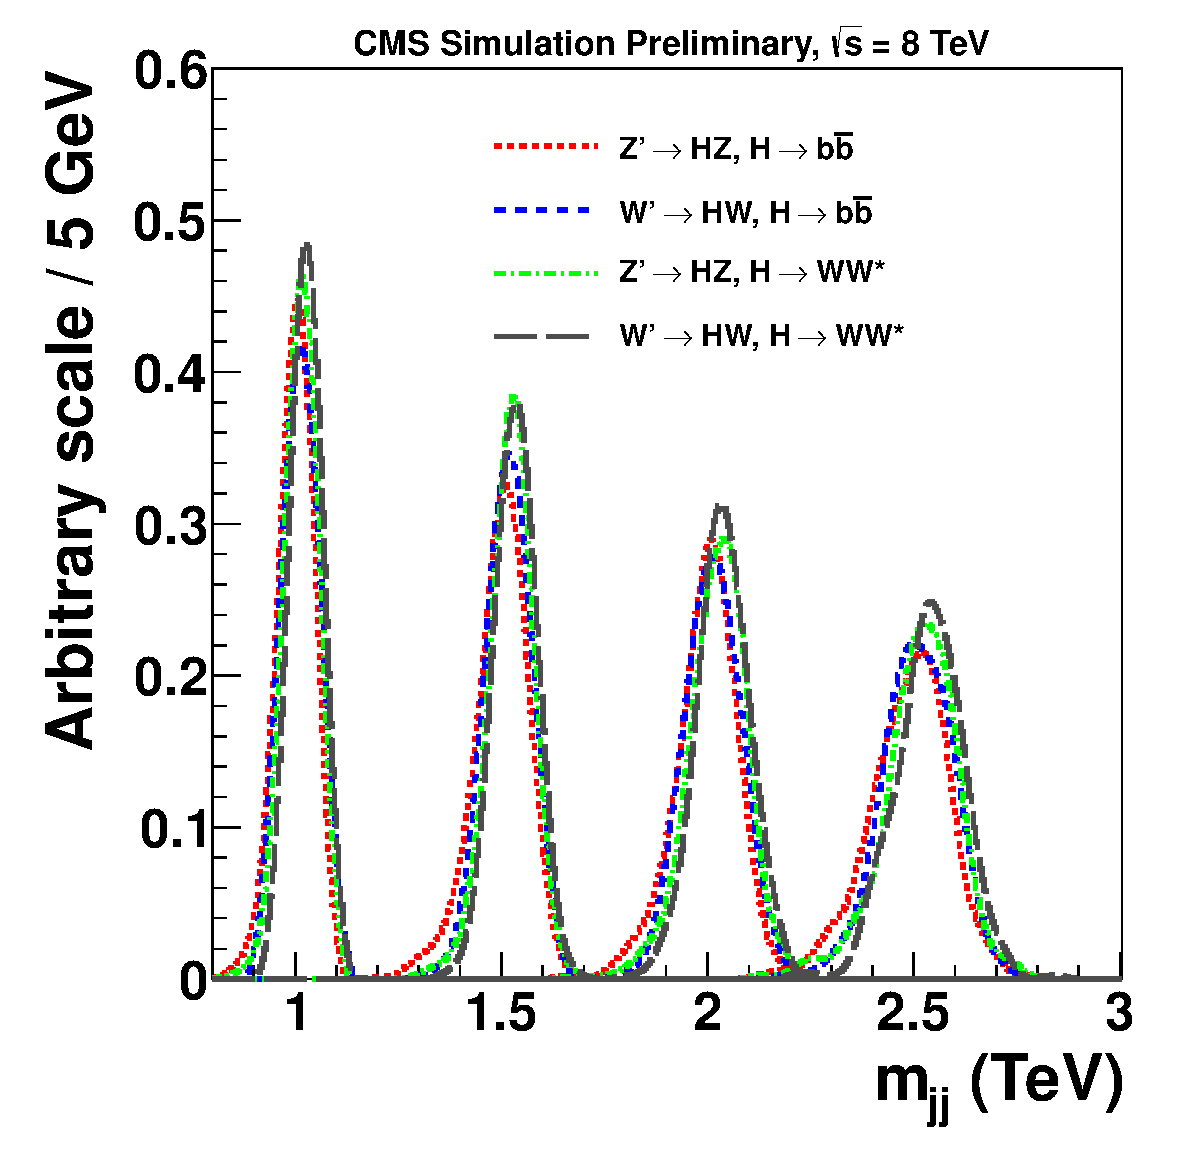
\includegraphics[width=0.7\textwidth]{EXO-14-009/shapeAll.pdf}
%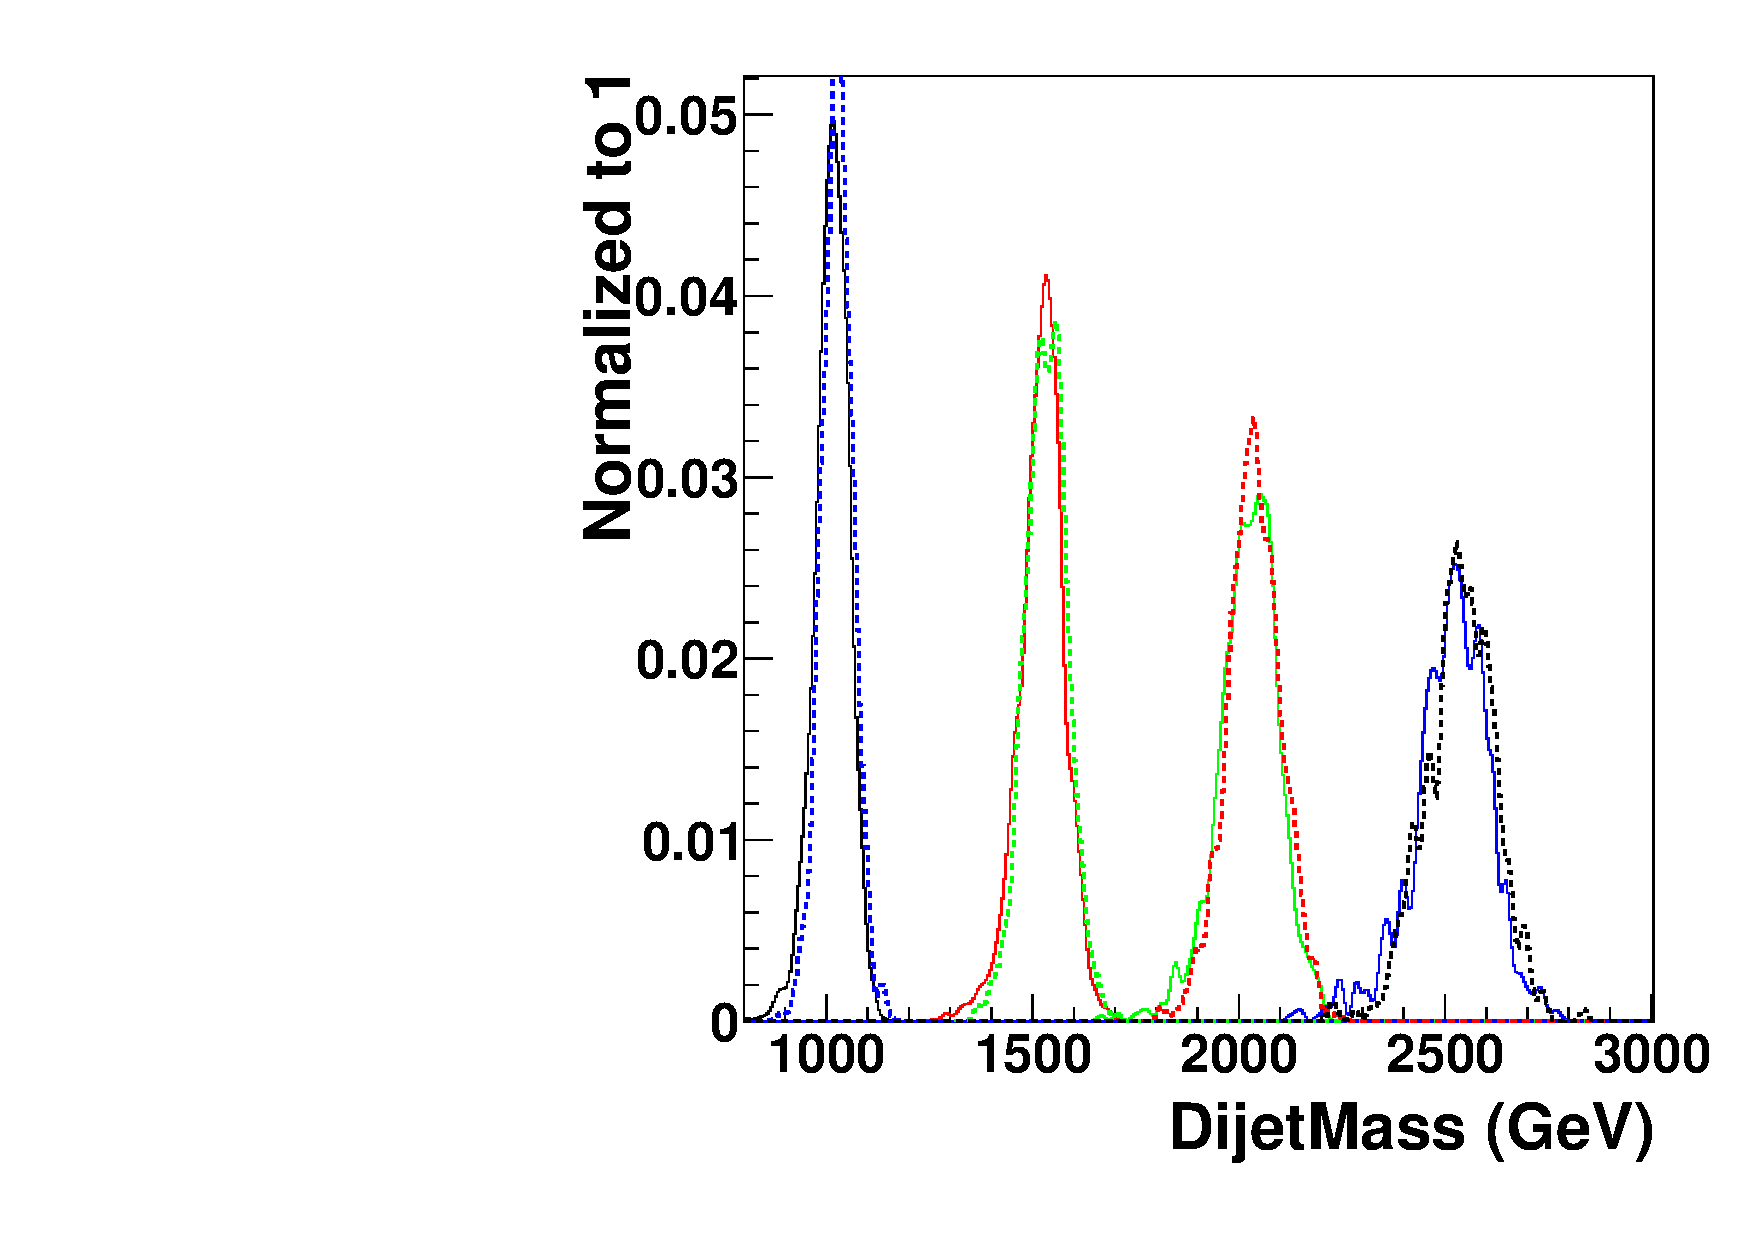
\includegraphics[width=0.49\textwidth]{HqqqqZqqfigs/Signal/shape.pdf}
\end{center}
\caption{Signal shapes for Z' and W' signals at 1.0, 1.5, 2.0 and 2.5 TeV
 resonances.
% Z' are shown in solid lines,
%W' are shown in dashed lines, in H(bb)V decay(left) and H(ww)V decay(right).
}
\label{fig:HbbZqqShape}
\end{figure}


%{\bf TO-DO: add the signal shapes here. and the overall signal tagging efficiency and data tagging efficiency.  }




\clearpage

